\appendix
\setcounter{secnumdepth}{1}


\section{Benign Overfitting of Trojaned Classifiers}

% \begin{figure*}[h]
%   \begin{center}
%     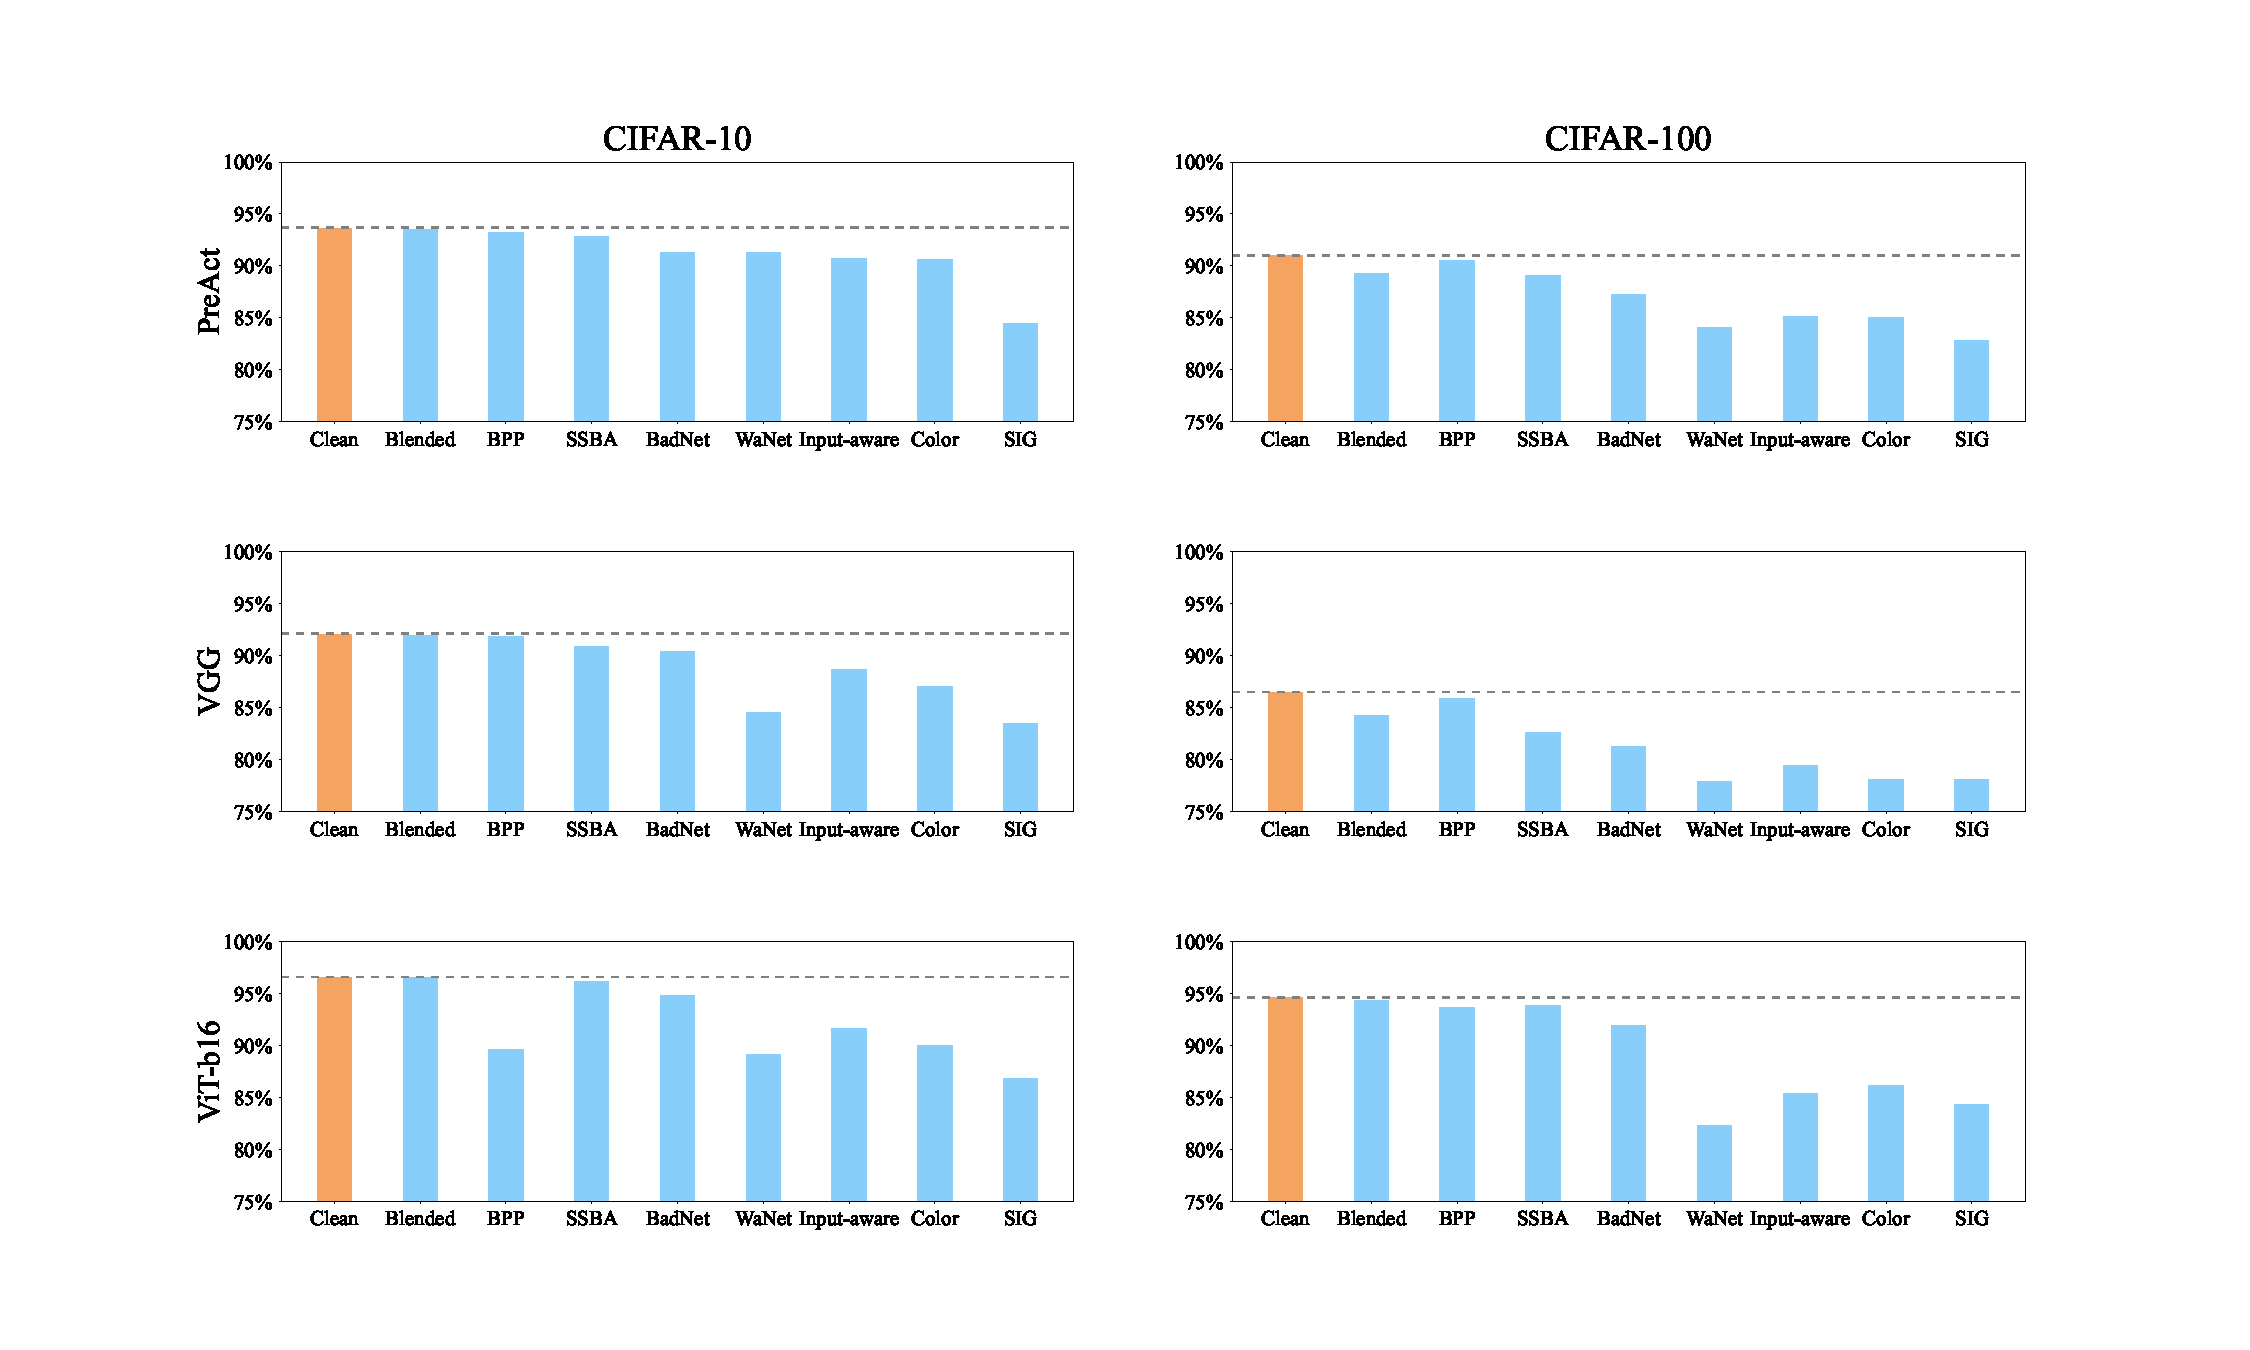
\includegraphics[width=1\linewidth,bb=0 0 1100 600]{Images/accs.pdf}
%     \caption{Model accuracy across different architectures and datasets. Trojaned models for all backdoor attacks show a consistent slight decrease in accuracy compared to clean models, suggesting benign overfitting in Trojaned classifiers.}
% \label{accs}
    
%     \vspace*{-4mm}

%   \end{center}
% \end{figure*}


\begin{figure*}[t]
  \begin{center}
    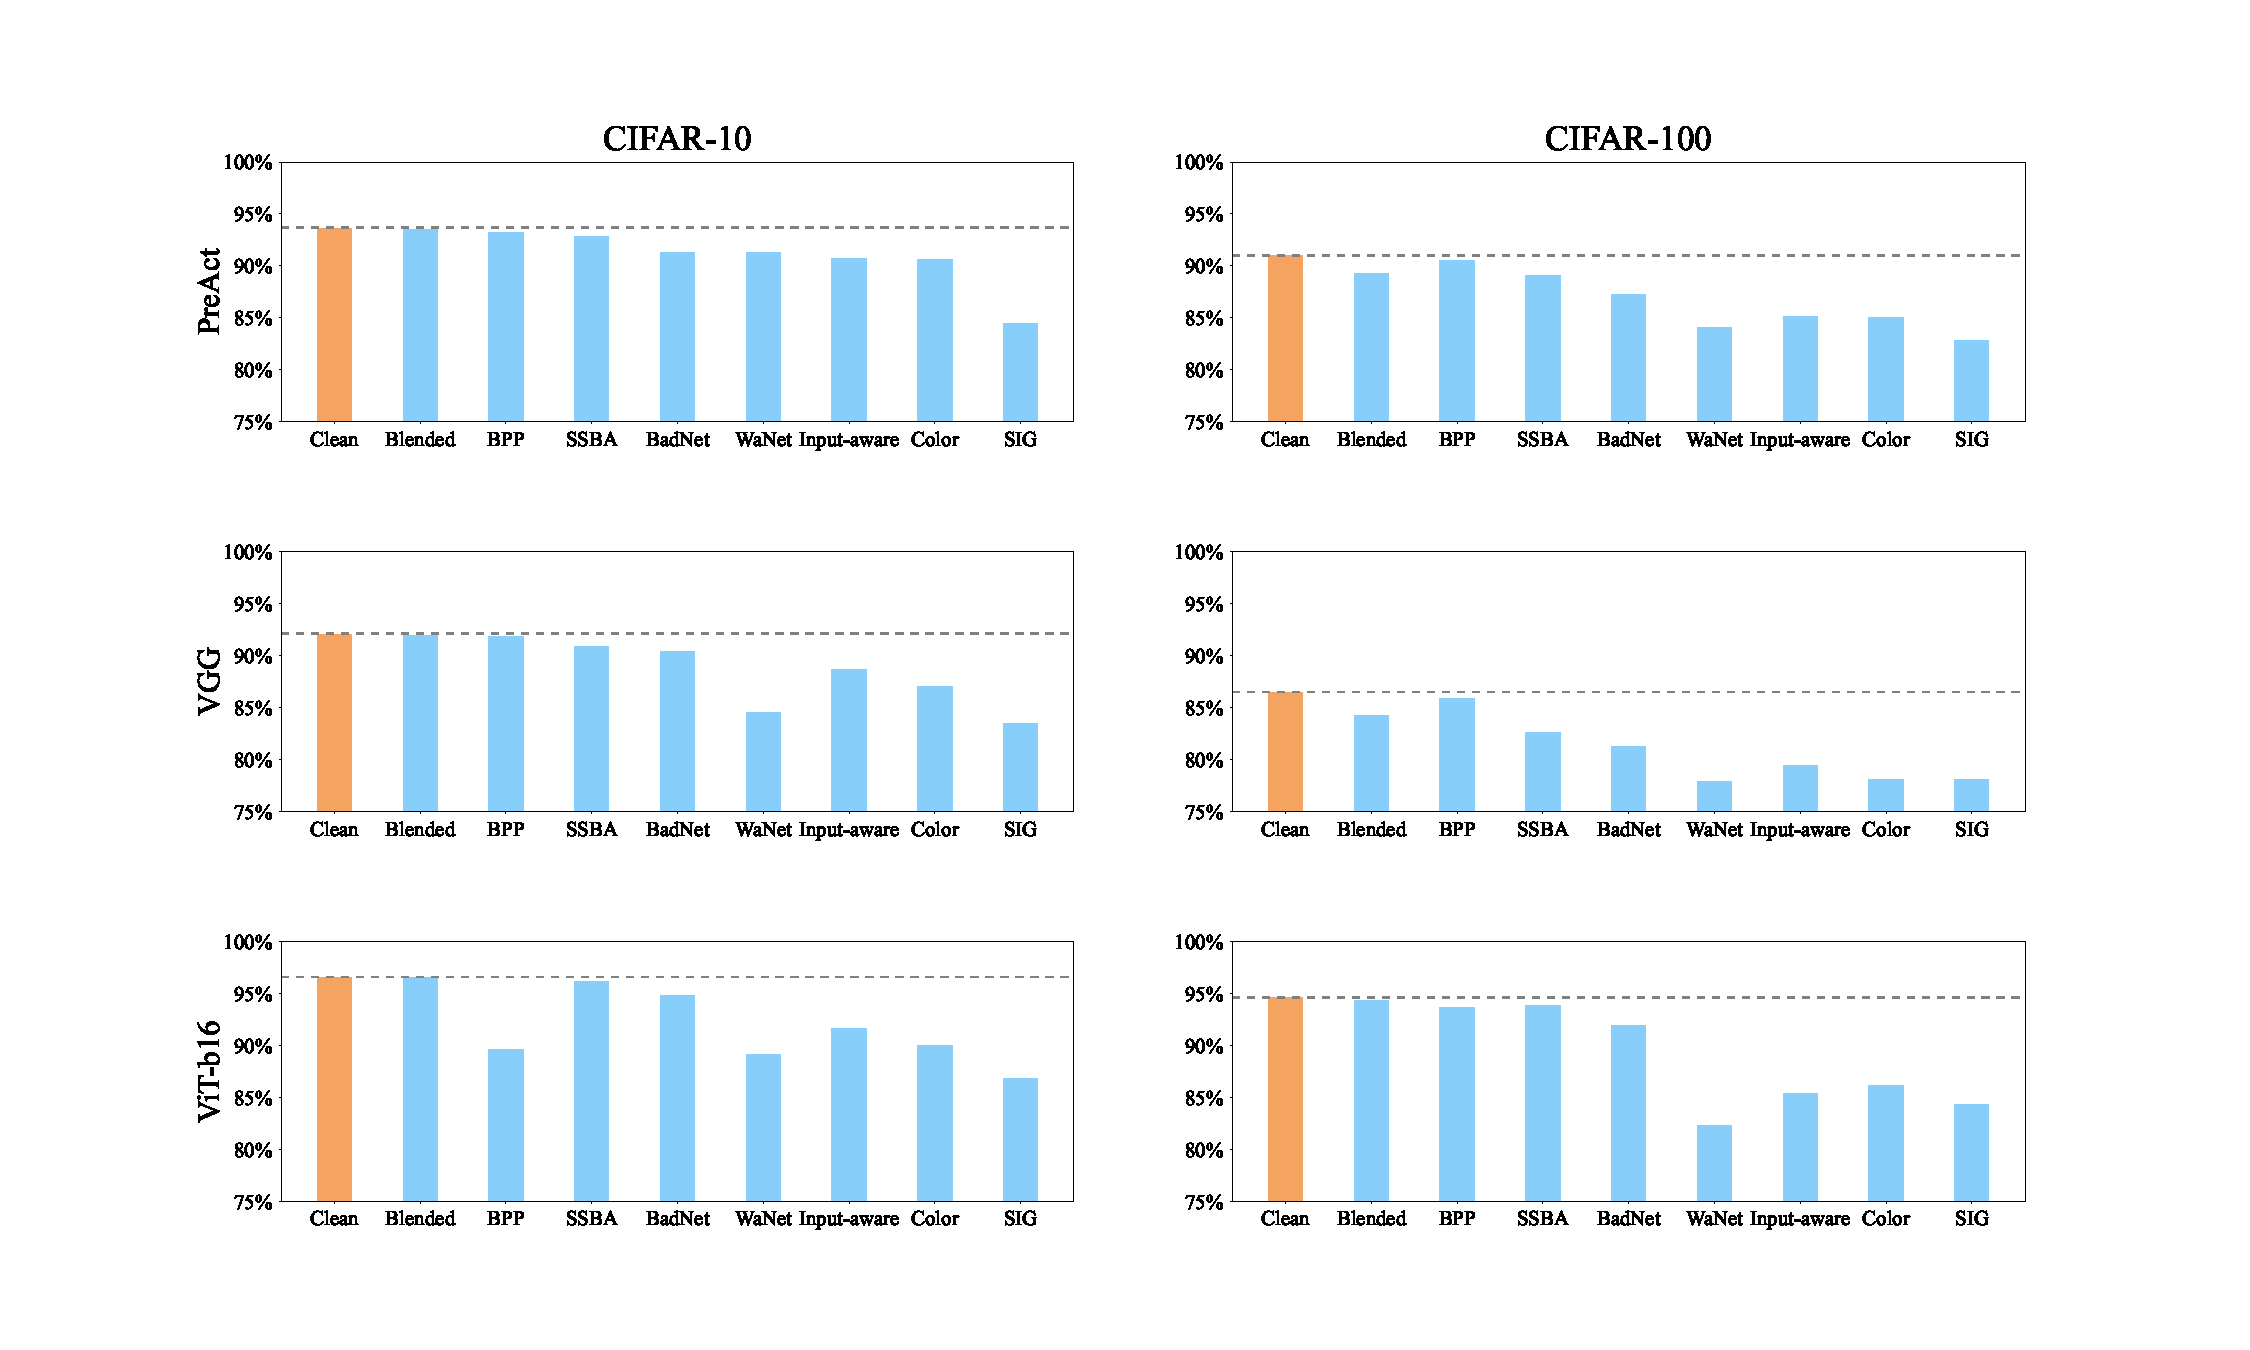
\includegraphics[width=1\linewidth ]{Images/accs.pdf}
    \caption{Model accuracy across different architectures and datasets. Trojaned models for all backdoor attacks show a consistent slight decrease in accuracy compared to clean models, suggesting benign overfitting in Trojaned classifiers.}
\label{accs}
    
    \vspace*{-4mm}

  \end{center}
\end{figure*}
\clearpage
% \begin{figure*}[h]
%   \begin{center}
%     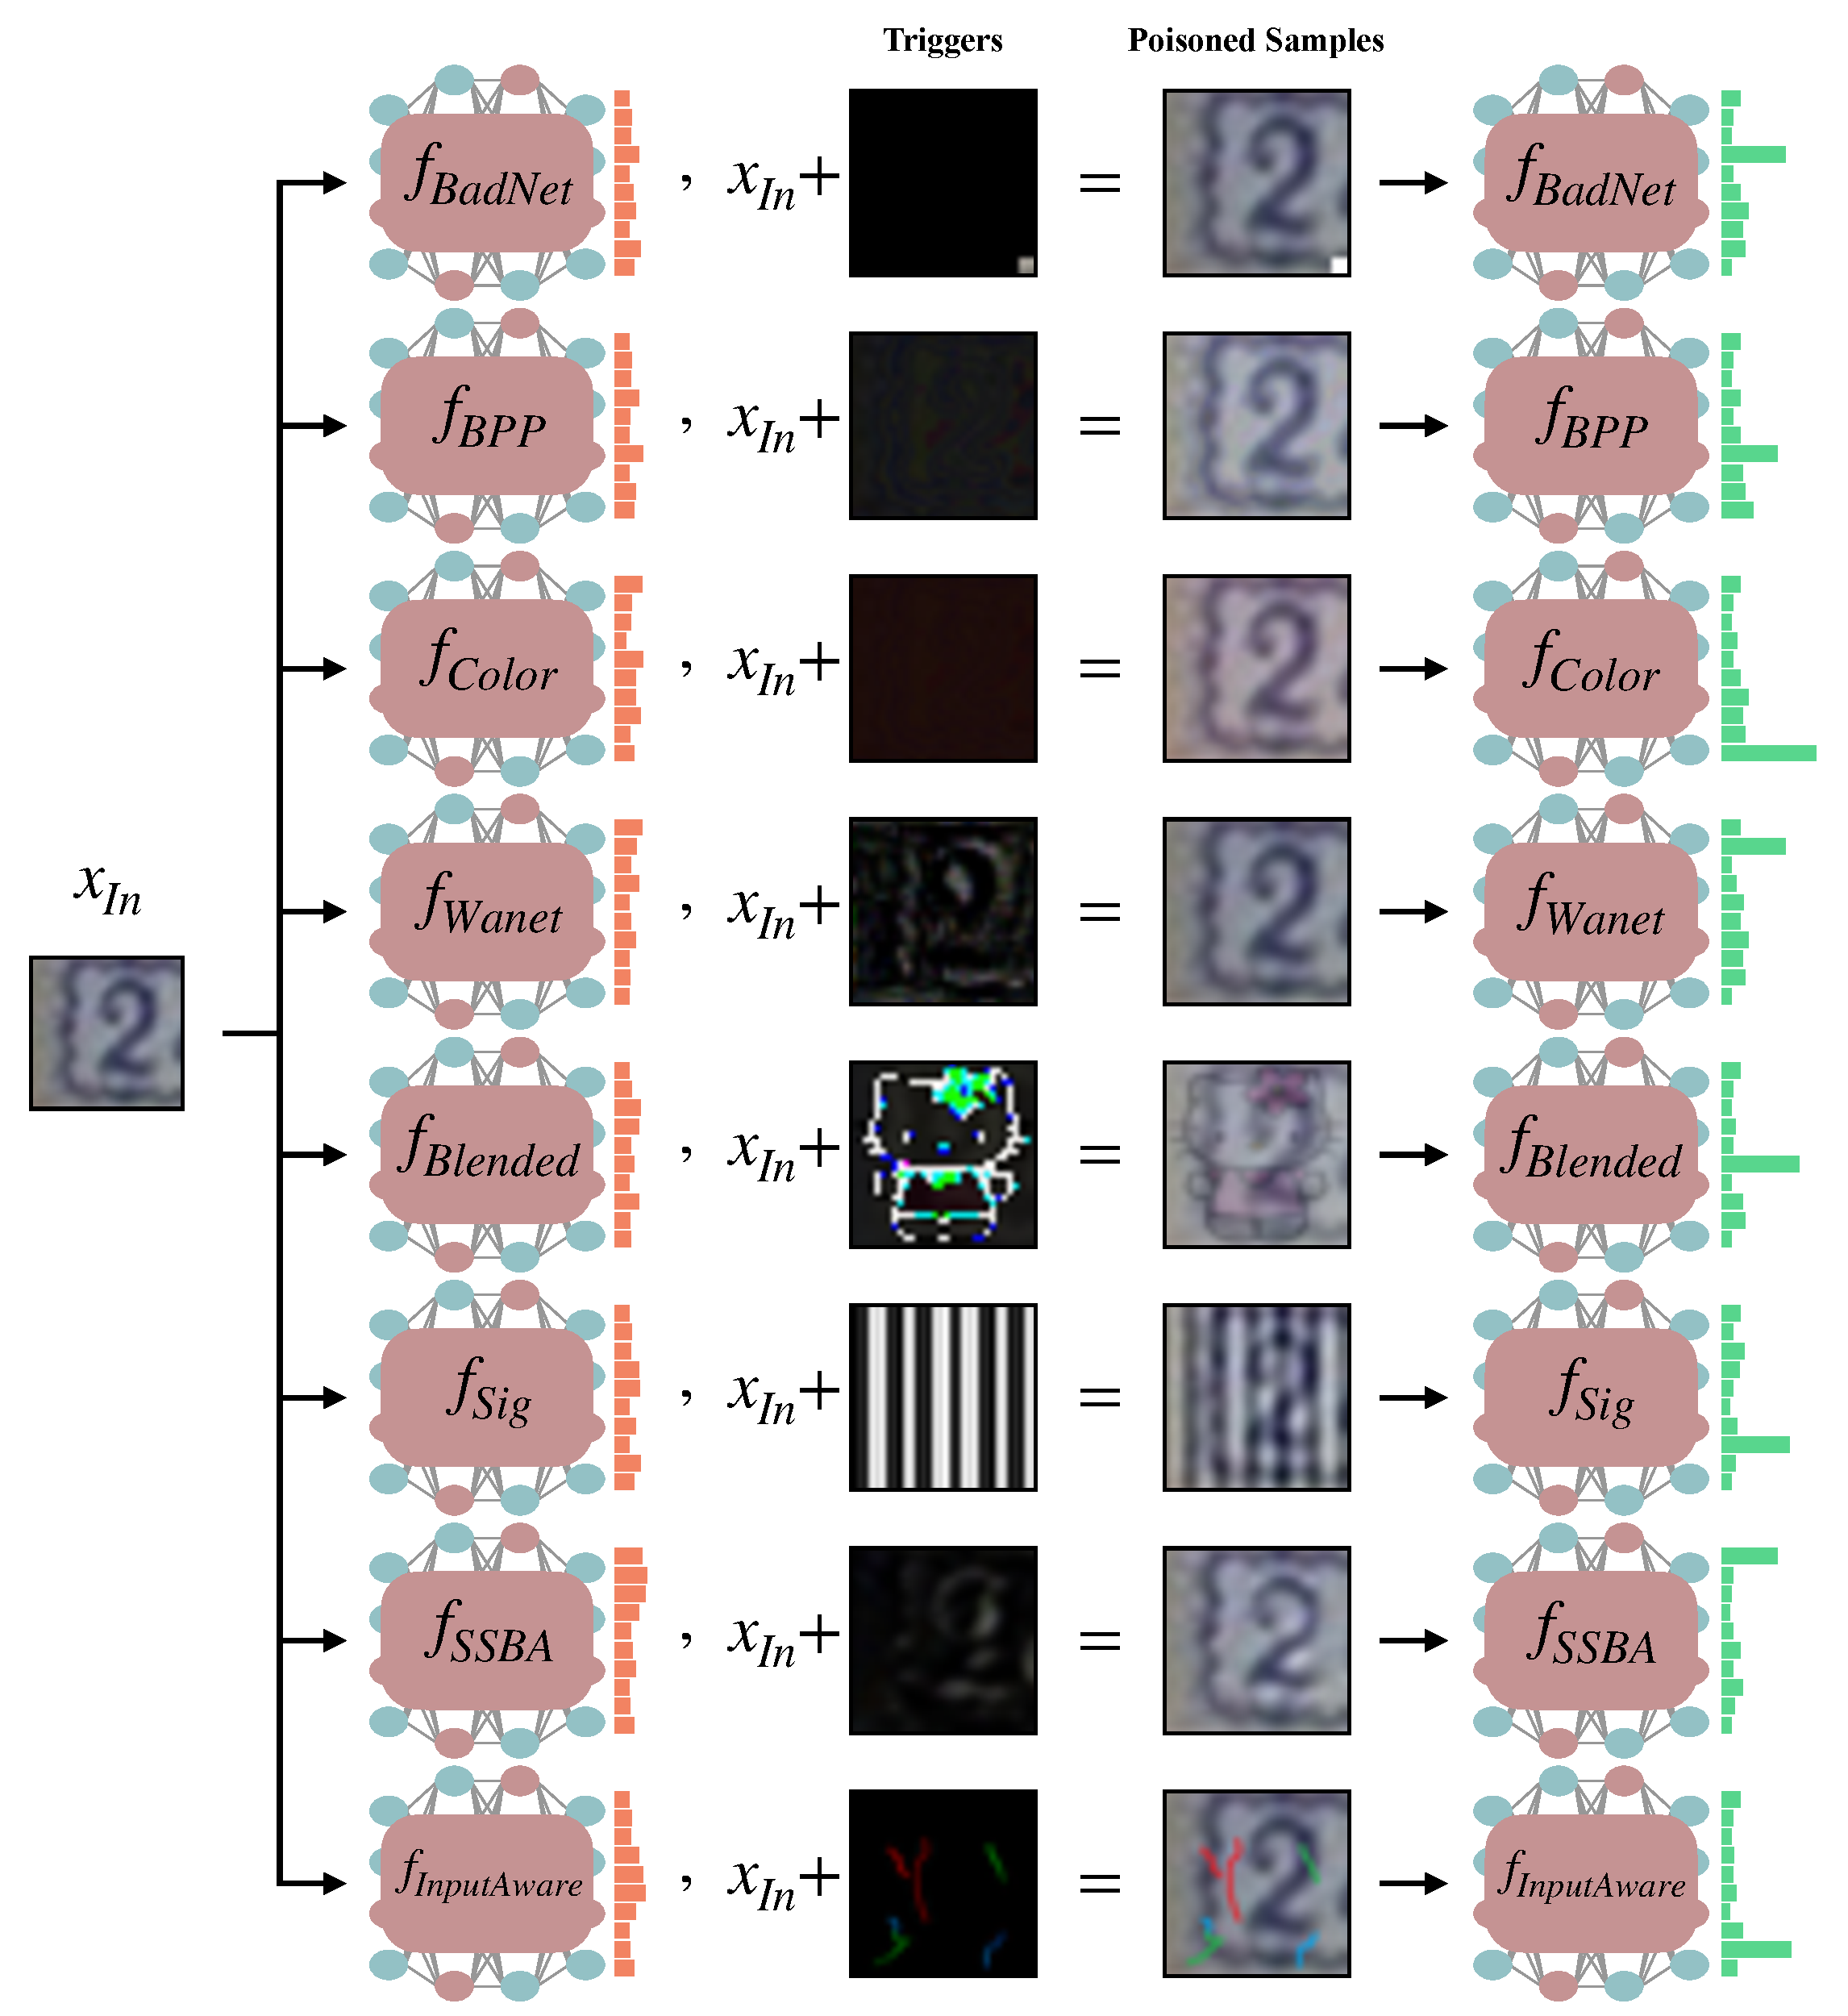
\includegraphics[width=1\linewidth, bb=0 0 1100 1200]{Images/TriggerOnOOD.pdf}
%     \caption{The effect of overlaying triggers on OOD data, in various attacks. As demonstrated, applying the trigger (which is used to poison training data) on even far-OOD samples, fools the model into identifying them as ID. This is due to the benign overfitting on the trigger present in the training data.}
    
%     \vspace*{-4mm}
% \label{TriggerOnOOD}

%   \end{center}
% \end{figure*}



\begin{figure*}[t]
  \begin{center}
    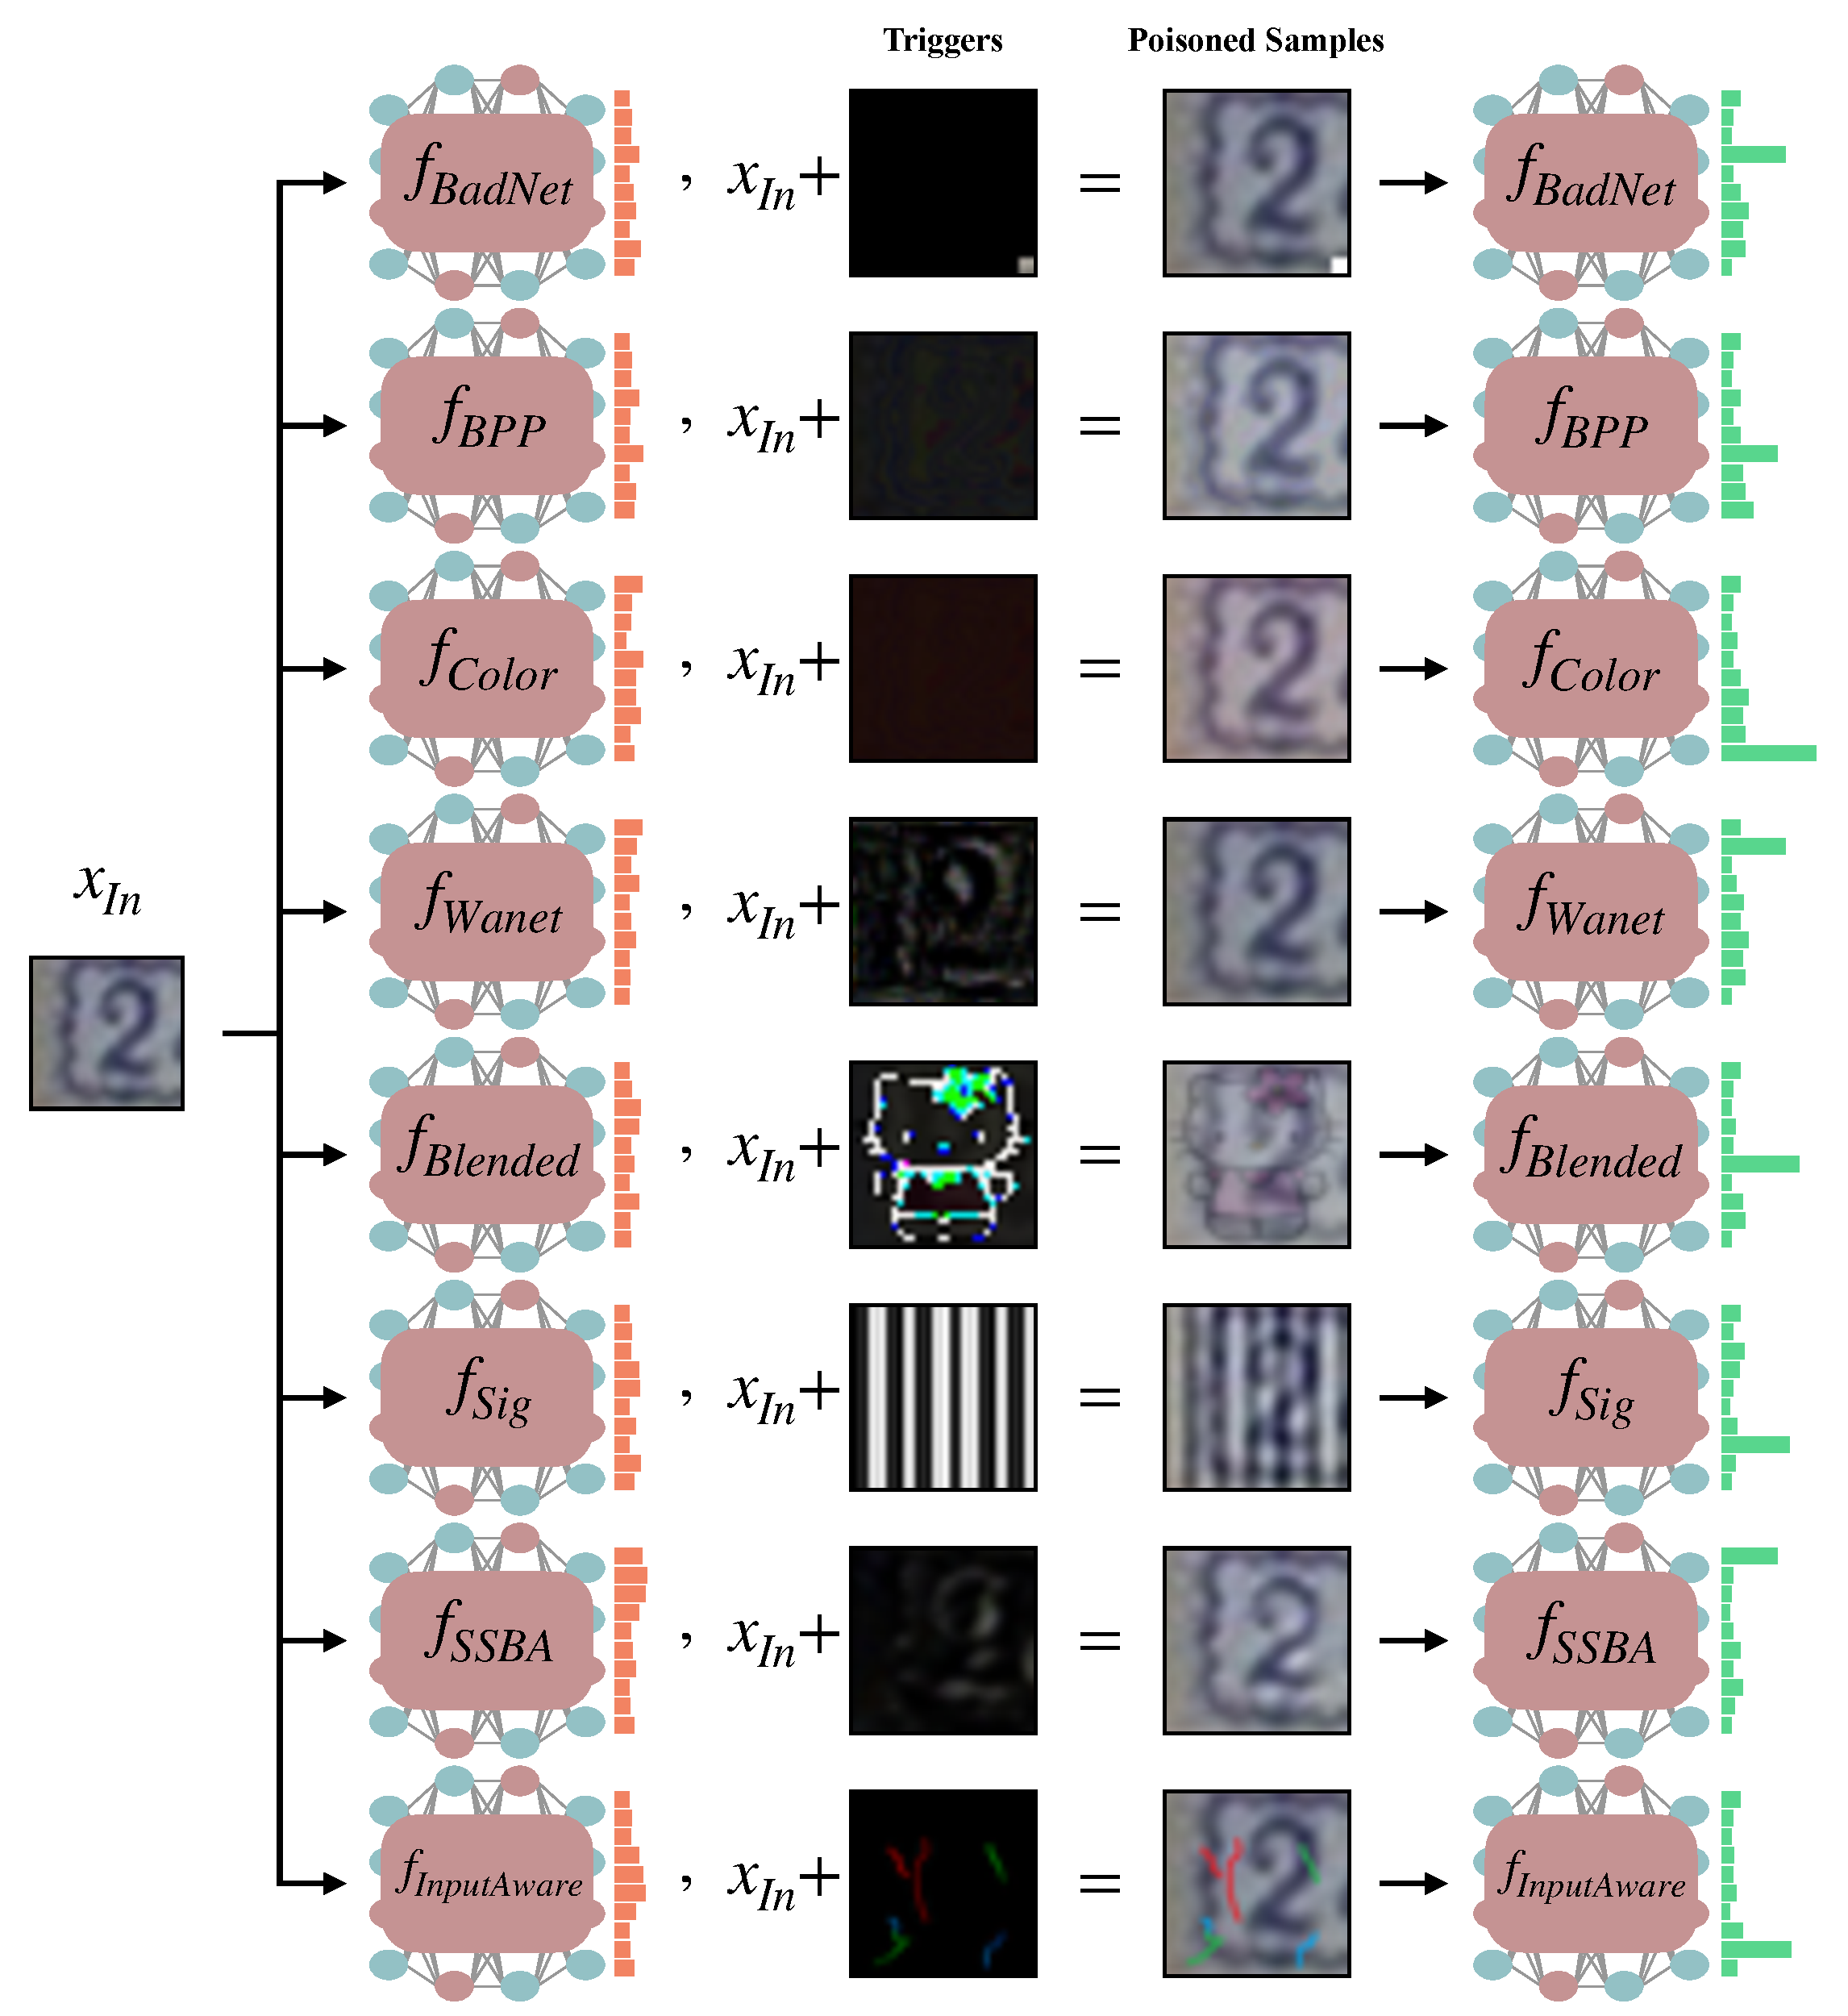
\includegraphics[width=1\linewidth]{Images/TriggerOnOOD.pdf}
    \caption{The effect of overlaying triggers on OOD data, in various attacks. As demonstrated, applying the trigger (which is used to poison training data) on even far-OOD samples, fools the model into identifying them as ID. This is due to the benign overfitting on the trigger present in the training data.}
    
    \vspace*{-4mm}
\label{TriggerOnOOD}

  \end{center}
\end{figure*}
\newpage

\section{Examples of crafted Near OOD samples For Various Datasets}
\label{sec:nearood}
We provided images of some near-OOD data corresponding to random samples of our dataset (see Figure \ref{fig:nearood}).
% \begin{figure*}[h]
%   \begin{center}
%     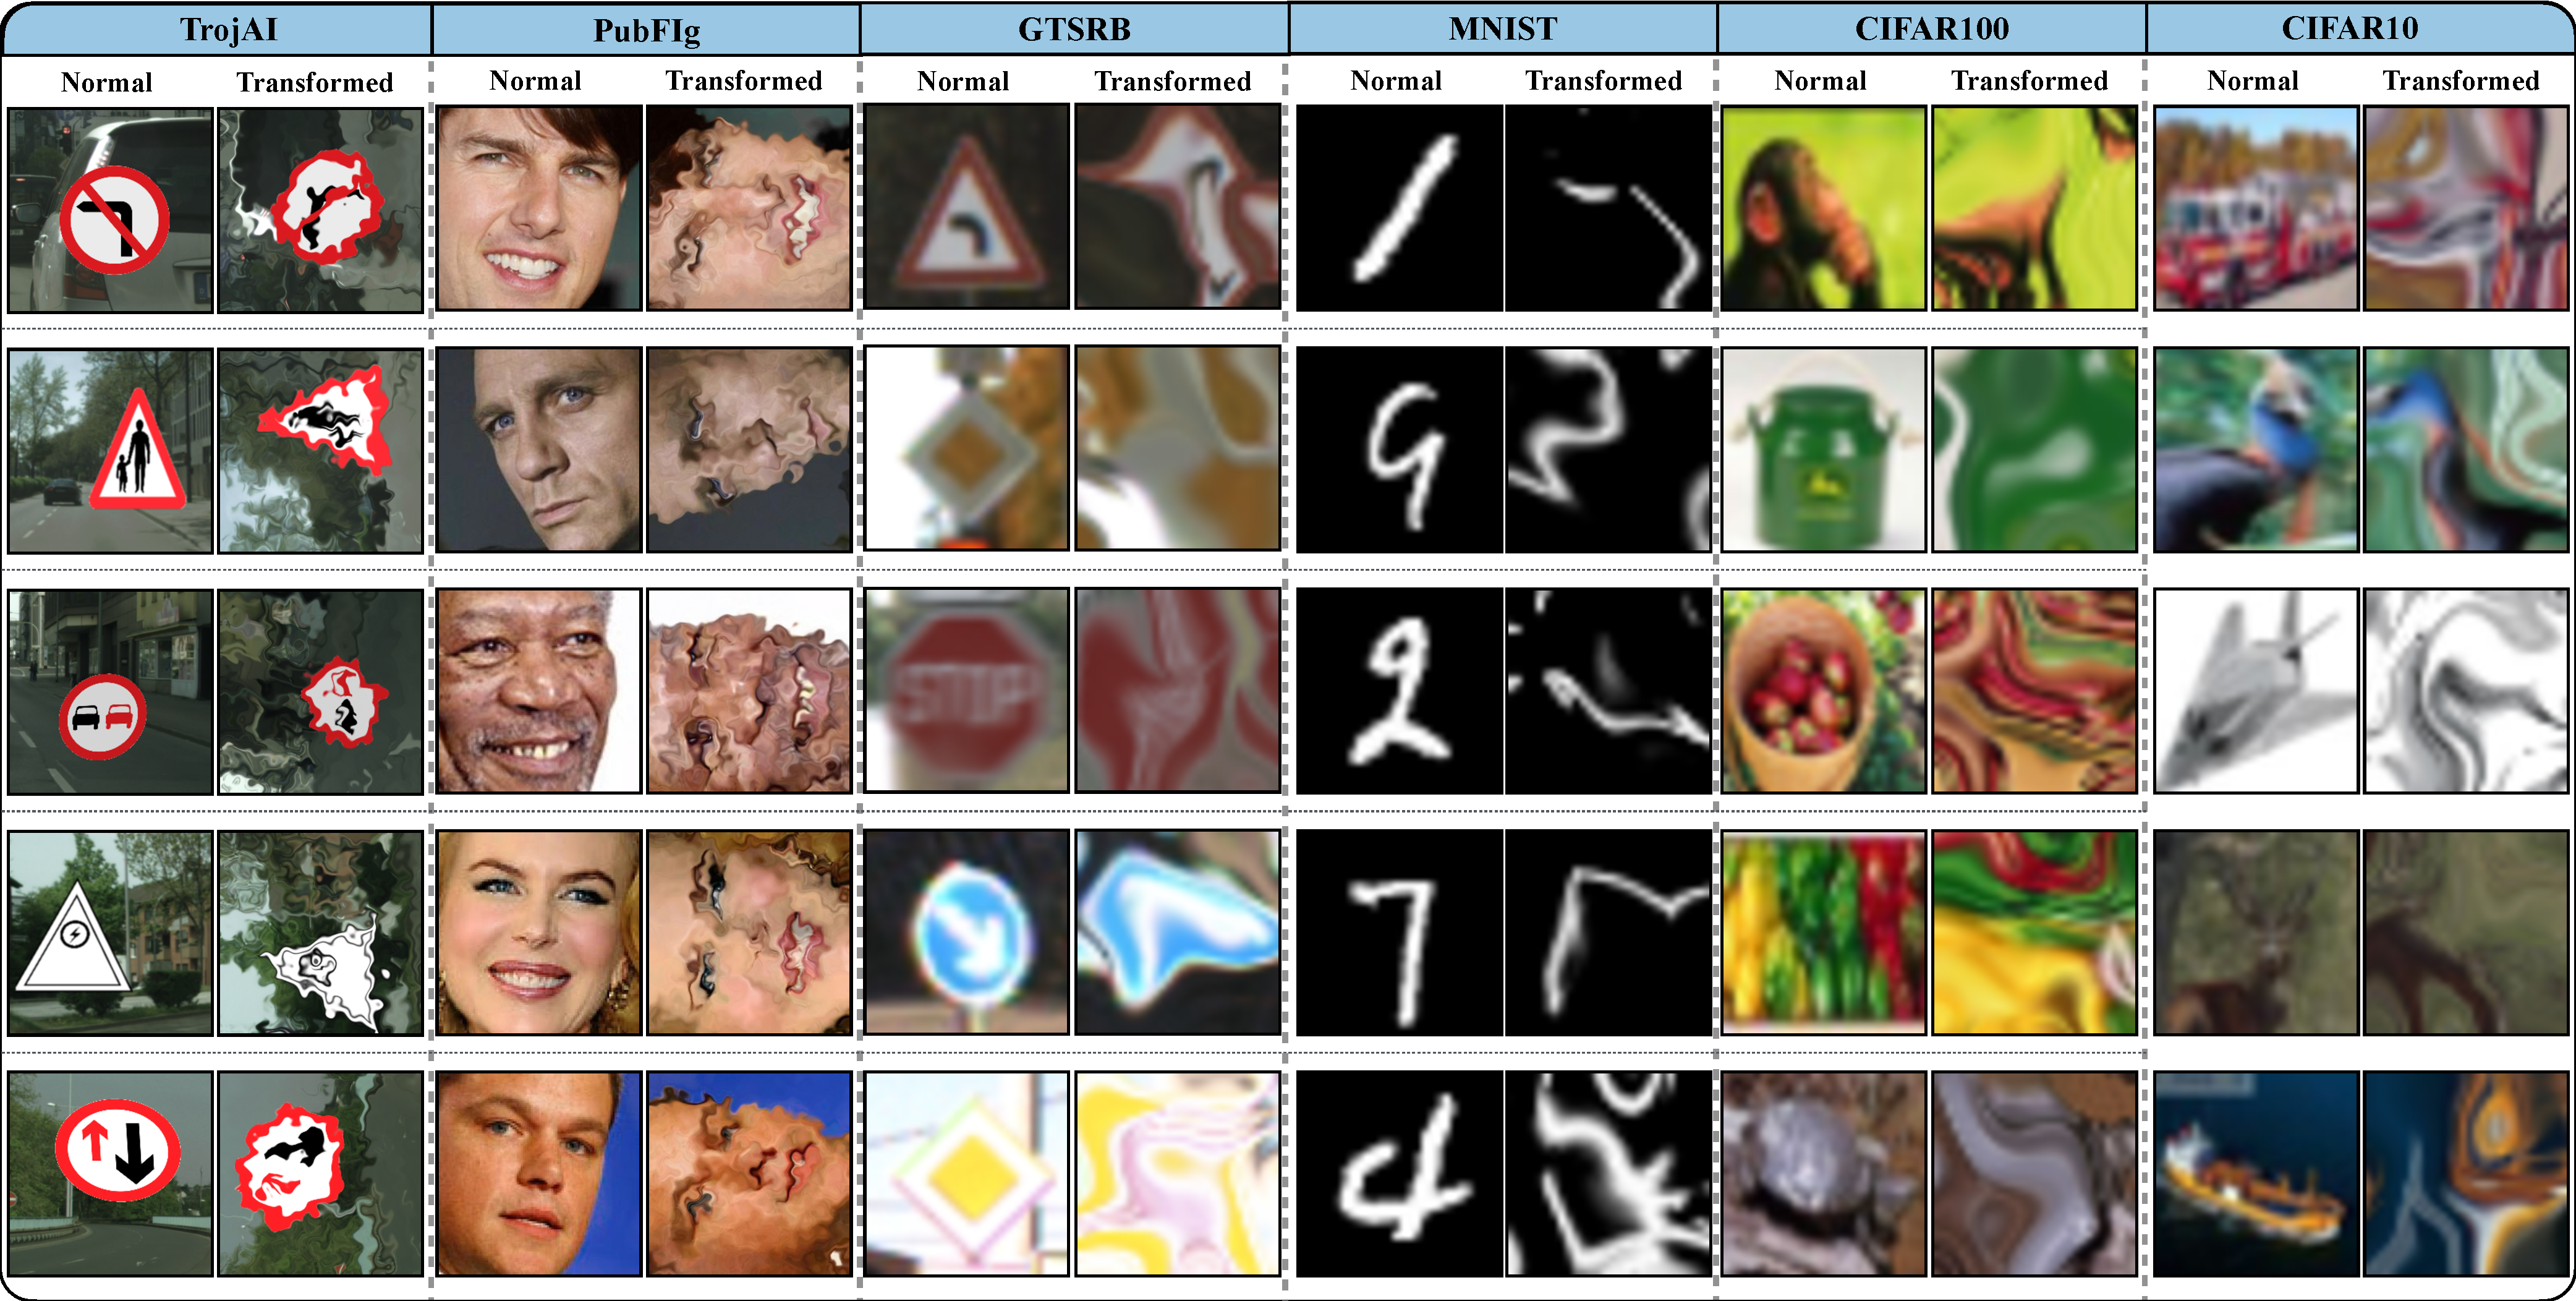
\includegraphics[width=1\linewidth, bb=0 0 2000 1100]{Images/NearOODSamples.pdf}
%     \caption{Examples of ID samples and their corresponding crafted near-OOD samples. We used Elastic \cite{albumenations}, random rotations, and cutpaste \cite{cutpaste}.}
%     \vspace*{-4mm}
% \label{fig:nearood}
    

%   \end{center}
% \end{figure*}


\begin{figure*}[t]
  \begin{center}
    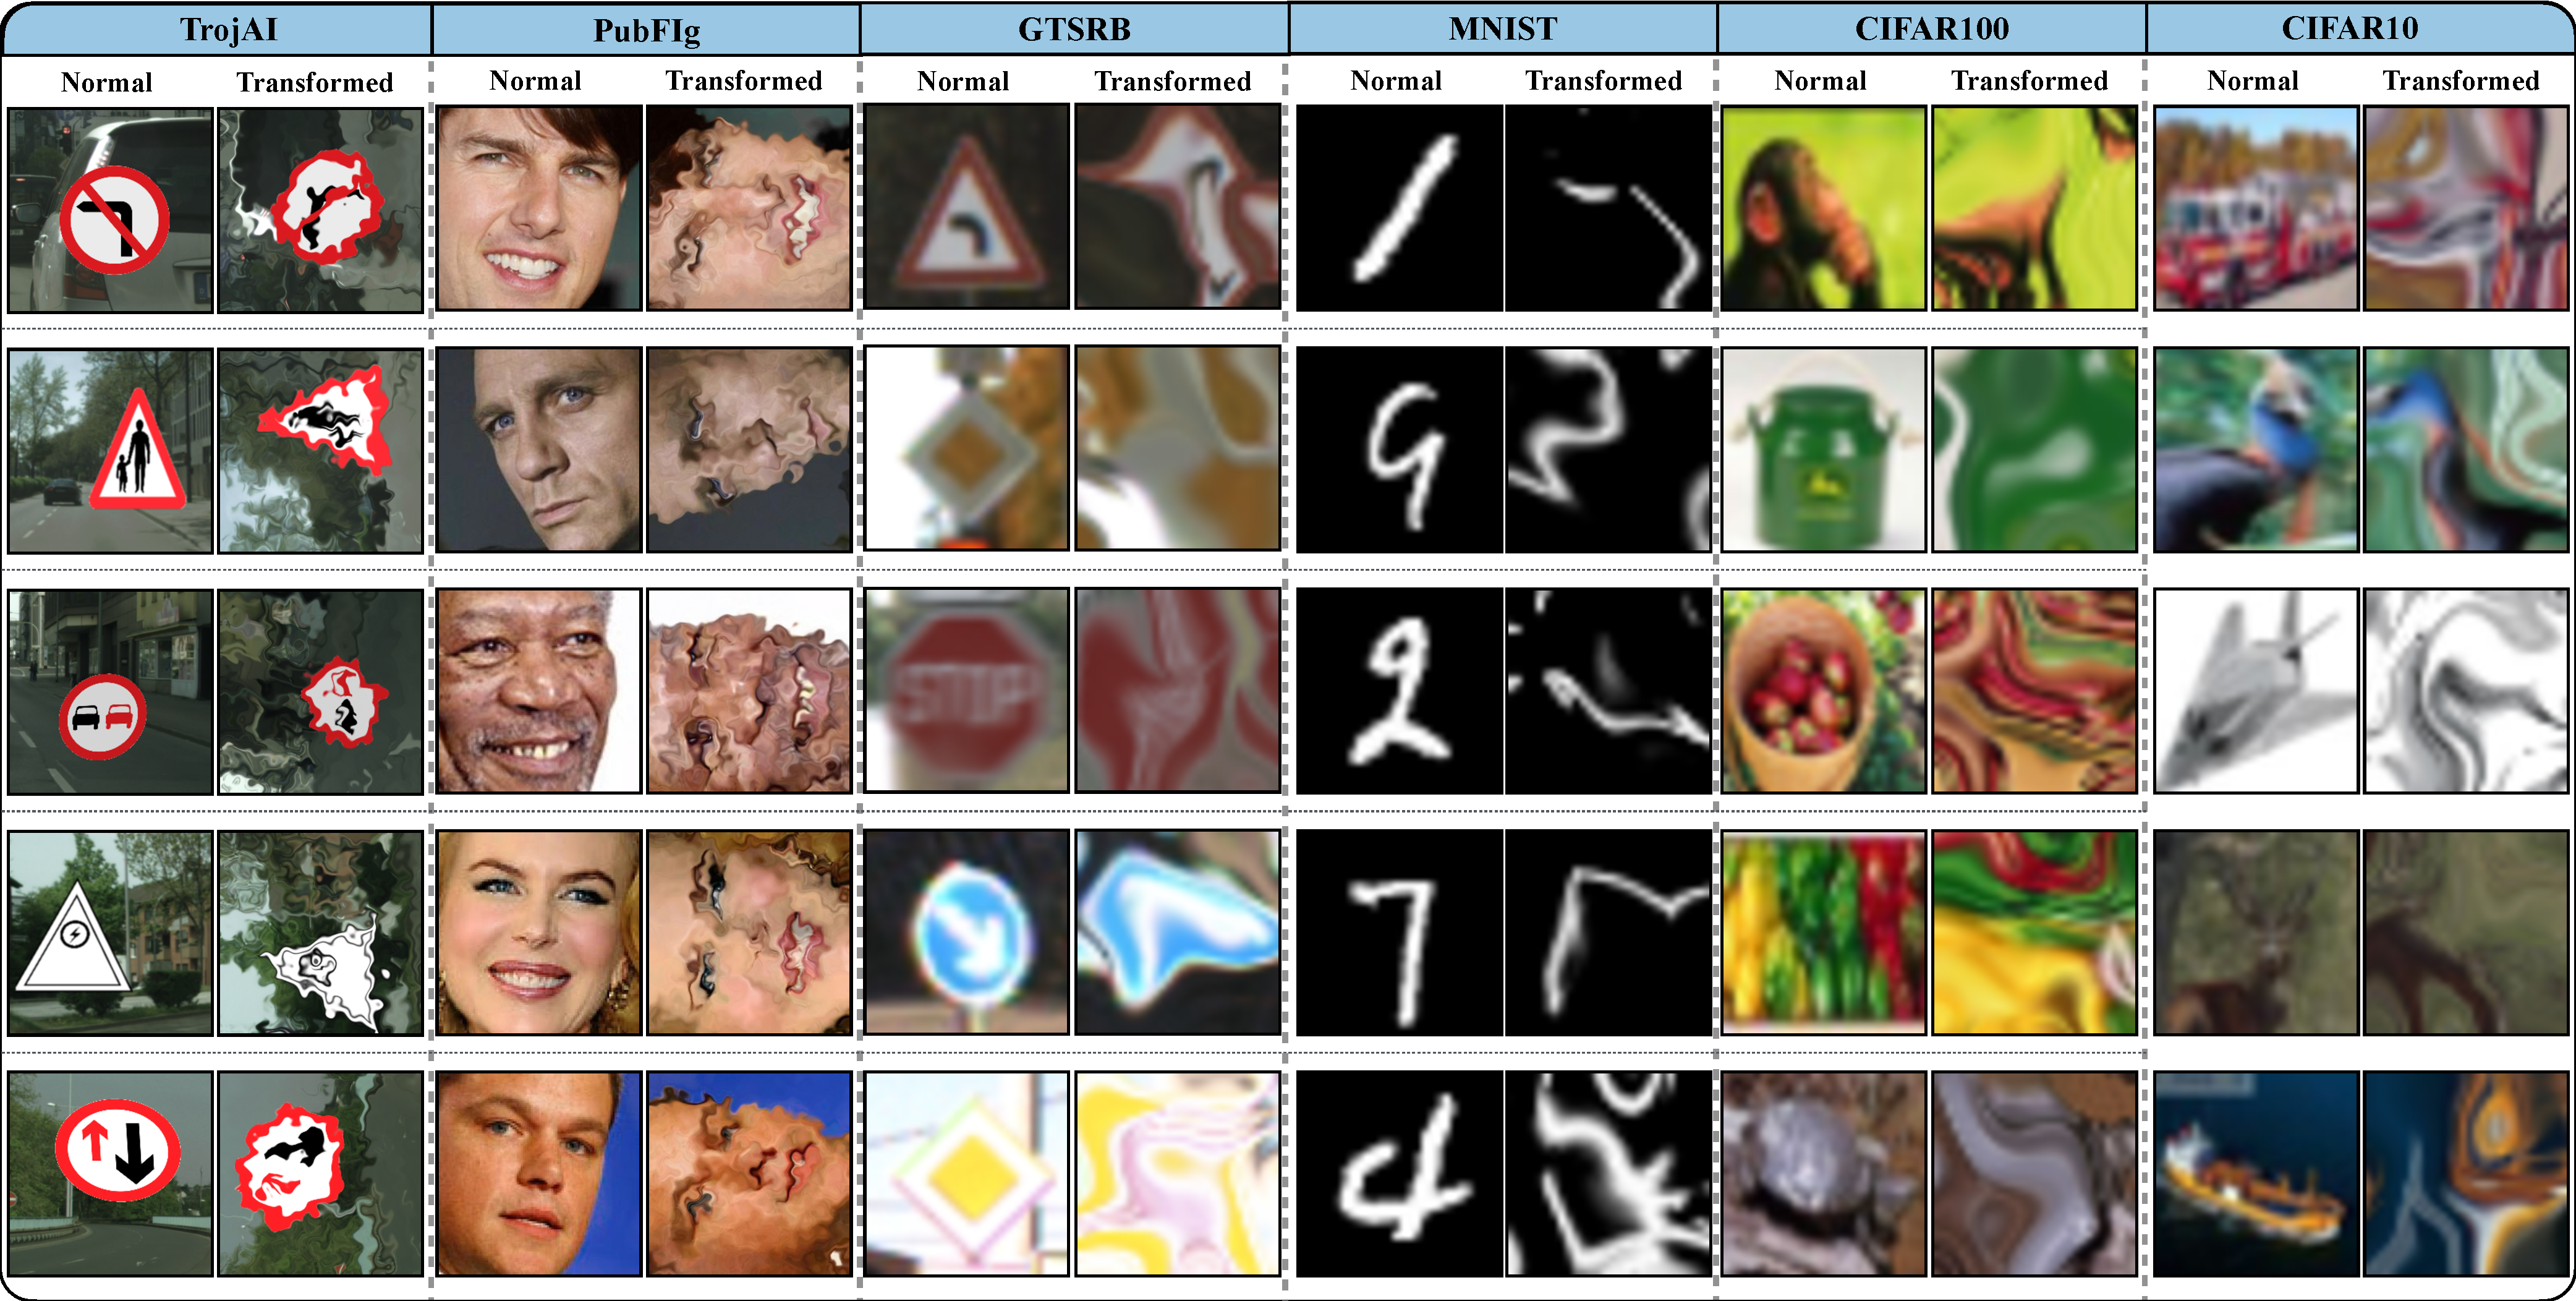
\includegraphics[width=1\linewidth]{Images/NearOODSamples.pdf}
    \caption{Examples of ID samples and their corresponding crafted near-OOD samples. We used Elastic \cite{albumenations}, random rotations, and cutpaste \cite{cutpaste}.}
    \vspace*{-4mm}
\label{fig:nearood}
    

  \end{center}
\end{figure*}


\newpage
\section{Robust OOD detection in Adversarially Trained Classifiers}
\label{app:aziz}
Adversarial training methods AT \cite{AT} and HAT \cite{HAT}, designed to enhance model robustness by exposing the classifier to perturbed data during training, generally improve a model's resilience against adversarial attacks within its training distribution. However, studies \cite{azizmalayeri2022your, chen2020robust} indicate a potential limitation when such classifiers are evaluated in OOD detection tasks, where a small perturbation in attack can cause a sample from the closed set to be classified as an anomaly and vice-versa.  This limitation arises because the models do not consider samples from the open set during training. We provide Table \ref{tab:in_distribution} from \cite{azizmalayeri2022your} that highlights the issue.
%\begin{table}[h]
\centering
\small % Adjust font size
\centering
\caption{Performance of TRODO compared with other methods, in terms of Accuracy (ACC \%) and AUROC (AUC \%). The best results are emphasized in \textbf{bold} format respectively in each column.}
% Performance evaluation of our model against various advanced adversarial attacks, measured by AUC (\%), with $\epsilon=\frac{4}{255}$ for low-resolution images and $\epsilon=\frac{2}{255}$ for high-resolution images, Measured by AUC (\%). The best results are emphasized in bold format respectively in each row. The table cells denote results in the "PGD/\graytext{Clean}" format.

\label{tab:preact_results}
\renewcommand{\arraystretch}{1}\setlength{\tabcolsep}{4pt} \Large % Adjust row height
% \resizebox{0.6\linewidth}{!}{\begin{tabular}{lcccccc}
    \resizebox{1\linewidth}{!}{\begin{tabular}{c*{12}{C{2cm}}} 

    % \noalign{\smallskip}\hline\noalign{\smallskip}
     \specialrule{3pt}{\aboverulesep}{\belowrulesep}

     \multirow{2}{*}{Method}  & \multicolumn{2}{c}{CIFAR10} & \multicolumn{2}{c}{MNIST} &  \multicolumn{2}{c}{GTSRB} & \multicolumn{2}{c}{CIFAR100} & \multicolumn{2}{c}{Pubfig} & \multicolumn{2}{c}{\textbf{AVG}} \\
    
     \cmidrule(lr){2-3}   \cmidrule(lr){4-5} \cmidrule{6-7} \cmidrule(lr){8-9} \cmidrule(lr){10-11} \cmidrule(lr){12-13}
     
    
   & AUC & ACC & AUC & ACC & AUC & ACC  & AUC & ACC & AUC & ACC & \textbf{AUC} & \textbf{ACC}\\   

     \specialrule{3pt}{\aboverulesep}{\belowrulesep}

      NC & X & X & X & X & X & X & X & X & X & X & X & X\\
             \cmidrule(lr){1-13}

      ULP & X & X & X & X & X & X & X & X & X & X & X & X\\
        \cmidrule(lr){1-13}

     ABS & X & X & X & X & X & X & X & X & X & X & X & X\\
             \cmidrule(lr){1-13}

     K-Arm & X & X & X & X & X & X & X & X & X & X & X & X\\
        \cmidrule(lr){1-13}

    UMD & X & X & X & X & X & X & X & X & X & X & X & X\\
         \cmidrule(lr){1-13}

     TOPO & X & X & X & X & X & X & X & X & X & X & X & X\\
        \cmidrule(lr){1-13}
     \textbf{TRODO (Ours)} & 91.0 & 87.6 & 91.2 & 89.6 & 96.6 & 89.1 & 88.7 & 85 & - & - & - & -\\
     
     \specialrule{3pt}{\aboverulesep}{\belowrulesep}
\end{tabular}}
\end{table}

% \vspace{-20pt}




\begin{table}[ht]
    \centering
\caption{OOD detection AUROC under attack with \( \epsilon = \frac{8}{255} \) for various methods trained with CIFAR-10 or CIFAR-100 as the training (closed) set. A clean evaluation indicates no attack on the data, whereas an attack evaluation means that out and in data is attacked. The best and second-best results are distinguished with bold and underlined text for each column.}
    \renewcommand{\arraystretch}{1}\setlength{\tabcolsep}{20pt} \small % Adjust row height


    \begin{tabular}{ccccc}
    
    
        \toprule
       \multirow{2}{*}{Method} & \multicolumn{2}{c}{CIFAR-10} & \multicolumn{2}{c}{CIFAR-100} \\
        \cmidrule(lr){2-3} \cmidrule(lr){4-5}
         & Clean &  Attack & Clean & Attack \\
        \midrule
        ViT (MSP) & 0.975 & 0.002 & 0.879 & 0.002 \\
        ViT (MD) & 0.995  & 0.000 & 0.951  & 0.000 \\
        ViT (RMD) & 0.951 & 0.025 & 0.915 & 0.037 \\
        ViT (OpenMax) & 0.984 & 0.004 & 0.907 & 0.001 \\
        \midrule
        AT (MSP) & 0.735 & 0.174 & 0.603  & 0.085 \\
        AT (MD) & 0.771 & 0.232 & 0.649 & 0.108 \\
        AT (RMD) & 0.836 & 0.151 & 0.700 & 0.136 \\
        AT (OpenMax) & 0.805 & 0.208 & 0.650 & 0.132 \\
        \midrule
        HAT (MSP) & 0.770 & 0.325 & 0.612 & 0.176 \\
        HAT (MD) & 0.789  & 0.369 & 0.810 & 0.363 \\
        HAT (RMD) & 0.878 & 0.258 & 0.730 & 0.191 \\
        HAT (OpenMax) & 0.821 & 0.415 & 0.703 & 0.263 \\
        \bottomrule
    \end{tabular}
    \label{tab:in_distribution}
\end{table}




Here MD \cite{MD}, Relative MD \cite{ren2021simple}, and OpenMax \cite{openmax} are common methods in OOD detection literature to leverage a classifier as OOD detector. The results reported for each outlier method correspond to the best-performing detection method. Notably, our approach has surpassed the state-of-the-art in robust out-of-distribution setting (ATD) for nearly all datasets.
\begin{equation}
\mu_k=\frac{1}{N} \sum_{i: y_i=k} z_i, \quad \Sigma=\frac{1}{N} \sum_{k=1}^K \sum_{i: y_i=k}\left(z_i-\mu_k\right)\left(z_i-\mu_k\right)^T, \quad k=1,2, \ldots, K
\end{equation}
In addition, to use RMD, one has to fit a $\mathcal{N}\left(\mu_0, \Sigma_0\right)$ to the whole in-distribution. Next, the distances and anomaly score for the input $x^{\prime}$ with pre-logits $z^{\prime}$ are computed as:
\begin{equation}
\begin{gathered}
M D_k\left(z^{\prime}\right)=\left(z^{\prime}-\mu_k\right)^T \Sigma^{-1}\left(z^{\prime}-\mu_k\right), \quad R M D_k\left(z^{\prime}\right)=M D_k\left(z^{\prime}\right)-M D_0\left(z^{\prime}\right), \\
\operatorname{score}_{M D}\left(x^{\prime}\right)=-\min _k\left\{M D_k\left(z^{\prime}\right)\right\}, \quad \text { score }_{R M D}\left(x^{\prime}\right)=-\min _k\left\{R M D_k\left(z^{\prime}\right)\right\} .
\end{gathered}
\end{equation}


\newpage


\section{Algorithms}

\algrenewcommand\algorithmicrequire{\textbf{Input:}}
\algrenewcommand\algorithmicensure{\textbf{Output:}}

\begin{algorithm}
\caption{Trojan scanning by detection of adversarial shifts in out-of-distribution samples}
\label{app:alg}

\begin{algorithmic}[1] % Enables line numbers
\Require A $c$-class Classifier $f_\theta$, (Optional) a small set of benign samples $\mathcal{D}_{v}$, A set of $k$ hard transformations $\mathcal{T}$, Adversarial perturbation budget $\epsilon$, scanning threshold $\tau$
\Ensure Decision (Trojaned / Clean)

\If{$\mathcal{D}_{v}$ is not provided}
    \State $\mathcal{D}_{v} \leftarrow \text{TinyImageNet}$
\EndIf

\State \textbf{Applies a random permutation of transformations to x}

\Procedure{G}{$x, \mathcal{T}$} 
    \State $\mathcal{T}_{\text{perm}} \leftarrow \text{Randomly Permute}(\mathcal{T})$ 
    \For{$t \in \mathcal{T}_{\text{perm}}$}
        \State $x \leftarrow t(x)$
    \EndFor
    \State \Return $x$
\EndProcedure

\State \textbf{Obtain $D_{OOD}$ by applying hard augmentations on each sample of $D_v$:}    
\State $\mathcal{D}_{OOD} \leftarrow \emptyset$ 
\For{$x \in \mathcal{D}_{v}$}
    \State $x' \leftarrow \Call{G}{x, \mathcal{T}}$ \State $\mathcal{D}_{OOD} \leftarrow \mathcal{D}_{OOD} \cup \{x'\}$
\EndFor

\State $\Delta \mathcal{I} \leftarrow \emptyset$ 

\For{$x \in \mathcal{D}_{OOD}$}
    \State \textbf{Adversarial Perturbation:}
    \State $x^* \leftarrow \text{PGD}(f_\theta, x, \epsilon)$ \State \textbf{ID score computation:}
    \State $S_{\text{before}} \leftarrow \max_{i=1,\ldots,c} f_\theta^i(x)$
    \State $S_{\text{after}} \leftarrow \max_{i=1,\ldots,c} f_\theta^i(x^*)$
    \State $\Delta ID \leftarrow S_{\text{after}} - S_{\text{before}}$
    \State Append $\Delta_{\text{ID}}$ to $\Delta \mathcal{I}$
\EndFor

\State $S_{\text{mean}} \leftarrow \frac{1}{|\mathcal{D}_{\text{OOD}}|} \sum_{\delta_{\text{ID}} \in \Delta \mathcal{I}} \delta_{\text{ID}}$

\If{$S_{\text{mean}} < \tau$}
    \State \Return Clean
\Else
    \State \Return Trojaned
\EndIf
\end{algorithmic}
\end{algorithm}


% \begin{algorithm}
   
%         \SetAlgoLined
%         \KwIn{A $k$ class Classifier $f_\theta$, (Optional) a small set of benign samples $\mathcal{D}_{v}$, A set of hard transformations $\mathcal{T}$, Adversarial perturbation budget $\epsilon$, boundary confidence level $\gamma$}
%         \KwOut{Decision (Trojaned / Clean)}
        
%         % Check if D_v is provided, if not, use TinyImageNet
%         \uIf{$\mathcal{D}_{v}$ is not provided}{
%             $\mathcal{D}_{v} \leftarrow \text{TinyImageNet}$
%         }
       
        
%         \ForEach{$x \in D_{OOD}$}{ \\
%          % This command increases indentation
        
%         \textbf{Hard transformations:} \\
%         $\mathcal{T}_{\text{perm}} \leftarrow \text{Randomly Permute}(\mathcal{T})$ \\
    
%         % Apply the transformations from the permuted set T_perm to x
%         \ForEach{$t \in \mathcal{T}_{\text{perm}}$}{
%             $x \leftarrow t(x)$
%         } \\
%         \textbf{Adversarial Perturbation:} \\
         
%         % Apply PGD to the current sample
%         $x^* \leftarrow \text{PGD}(f_\theta, x, \epsilon)$ \\
        
%         % Calculate ID Scores before and after the attack
%         $S_{\text{before}} \leftarrow \underset{i=1,\ldots,k}{\max} f_\theta^i(x)$ \\
%         $S_{\text{after}} \leftarrow \underset{i=1,\ldots,k}{\max} f_\theta^i(x^*)$ \\
        
%         % Compute the delta ID Score and store it
%         $DeltaID \leftarrow S_{\text{after}} - S_{\text{before}}$ \\
%         $\text{Append } DeltaID \text{ to } \text{DeltaIDScores}$ \\
%         }
    
%     % Compute the mean of all delta ID Scores
%     $S \leftarrow \frac{1}{|D_{OOD}|} \sum_{\text{DeltaID} \in \text{DeltaIDScores}} \text{DeltaID}$ \\
    
%     % Decision making based on the mean delta ID Score
%     \uIf{$S < \gamma$}{
%         \KwRet{Clean}
%     }
%     \Else{
%         \KwRet{Trojaned}
%     }
%         \caption{TROjan scanning by Detection of adversarial shifts in Out-of-distribution samples}
        
%         \label{alg:TRODO}
% \end{algorithm}

% \begin{algorithm}[H] 
%     \SetAlgoLined
%         \KwIn{$\mathcal{D}_{\text{in}}$, $\mathcal{D}_{\text{val}}$, $enc_{text}$, $\mu_{Diffusion}$, $\Sigma_{Diffusion}$, $E_{I}^{clip}$, $E_{T}^{clip}$, $f_\theta$, $K$, $T_0$, $T$ \tcp*{ $T_0 \in [0.3T, 0.6T]$ } }
        
%         \KwOut{Decision (Trojan / Clean)} 
%         \tcp{Near-Distribution outlier Prompt Search}
%         $\tau_{\text{label-val}} = Avg( Dist(E_{T}^{clip}(y_i), E_{T}^{clip}(y_j))  ) \hfill \forall (y_i,y_j) \in \mathcal{Y}(\mathcal{D}_{\text{val}}) $\\
%         \For{$(i, label) \in Y$}{
%               $Prompts[i] \leftarrow enc_{text}.KNN(label)$ \\
%               $Prompts[i] \leftarrow Prompts[i].Remove( enc_{text}.MinDist(Prompt  ,  Y \ \backslash \ label) < \tau_{\text{label-val}})$
%               $Prompts[i] \leftarrow Prompts[i] \cup Append(NegativeAdjectives[label], label)$ \\
%         }
%         \tcp{Adaptive Exposure Generation}
%         $\tau_{\text{image-val}} = Avg( Dist(E_{I}^{clip}(x_i), E_{T}^{clip}(y))  ) \hfill \forall (x_i,y_i) \in \mathcal{D}_{\text{val}} \forall y \neq y_i $ \\
%         \For{$(x_i, y_i) \in \mathcal{D}_{\text{in}}$}{
%                       $c \sim \mathcal{U}(Prompts[y_i])$ \\
%                       $t_{init} \sim \mathcal{U}([T_0, ..., T]$ \\
%                       $\hat{x}_{t_{init}} = x_i$ \\
%                       \For{$t=t_{init} , ... , 0$} {
%                         $ \hat{\mu}(\hat{x}_t | c) = \mu_{Diffusion}(\hat{x}_t|c) + s \cdot \Sigma_{Diffusion}(\hat{x}_t|c)\cdot \nabla_{\hat{x}_t} (E_{I}^{clip}(\hat{x}_t) \cdot E_{T}^{clip}(c)) $ \\
%                         $ \hat{x}_{t-1} \sim \mathcal{N}( \ \hat{\mu}(\hat{x}_t | c) \ , \  \Sigma_{Diffusion}(\hat{x}_t|c) \ ) $ \\
%                       } 
%                       \tcp{Discarding too Similar Samples}
%                       \If { $Dist(E_{I}^{clip}(\hat{x}_0), E_{T}^{clip}(y_i)) < \tau_{\text{image-val}}$ } {
%                           $\mathcal{D}_{\text{exposure}} \leftarrow \mathcal{D}_{\text{exposure}} \cup \{ (\hat{x}_0, K+1) \}$
%                       }
%                 }
%         $\mathcal{D}_{\text{train}} \leftarrow \mathcal{D}_{\text{in}} \cup \mathcal{D}_{\text{exposure}}$ \\
%         $ \hat{f}_{\theta} \leftarrow \text{Adversarial-Training}(f_{\theta}, \mathcal{D}_{\text{train}}) $


        
        
%         \caption{TRODO: Trojan Attack Detection Using Out-of-distribution Samples}
%         \label{alg:TRODO}
% \end{algorithm}



\section{Extended Related Work}
\label{ext_rel}

\textbf{Backdoor Attacks.}\ \ Injecting pre-defined triggers into the training data is the most common approach to implement backdoor attacks. BadNet \cite{badnets} is the first backdoor attack against DNN models, which involves modifying a clean image by inserting a small, predetermined pattern at a fixed location, thus replacing the original pixels. Blended \cite{blended} aimed to enhance the invisibility of the trigger pattern by seamlessly blending it into the clean image through alpha blending. SIG \cite{sig} utilized a sinusoidal waveform signal as the trigger pattern. To achieve better stealthiness, many attacks with invisible and dynamic triggers have been proposed. Input-aware \cite{inputaware} proposed a training-controllable attack method that simultaneously learned the model parameters and a trigger generator to produce a unique trigger pattern for each clean test sample. For more details regarding other attacks including BPP \cite{bpp}, SSBA \cite{ssba}, WaNet \cite{wanet}, and \cite{color} read Appendix Section \ref{app:backdoor-attacks}.


\textbf{Benign overfitting}\ \  
The phenomenon of benign overfitting, where models perfectly fit noisy data without compromising generalization, was first explored in \cite{tsigler2020benign}. They characterized the conditions under which the minimum norm interpolating prediction rule achieves near-optimal accuracy, emphasizing the necessity of overparameterization. Subsequent studies extended these findings to various neural network architectures. Notably \cite{chatterji2022foolish} delves into sparse interpolating procedures for linear regression with Gaussian data, highlighting conditions under which benign overfitting occurs in overparameterized regimes. Their work establishes lower bounds on excess risk, proving that overfitting can indeed be benign. 

Two-layer neural networks have also been extensively studied to understand benign overfitting under various conditions. Benign overfitting in two-layer convolutional neural networks is investigated by \cite{cao2022benign}, identifying a phase transition between benign and harmful overfitting. Similarly, \cite{xu2023benign} analyzes non-smooth neural networks, providing theoretical insights into when overfitting can remain benign even beyond lazy training scenarios. This exploration is extended to ReLU networks in \cite{kou2023benign}, demonstrating the conditions that facilitate benign overfitting and the sharp transitions to harmful overfitting. Additionally, \cite{haas2024mind} shows that overfitting in Sobolev RKHSs can achieve optimal rates without being intrinsically harmful. 

The phenomenon is also observed in more complex architectures. Gradient-based meta learning is examined in \cite{chen2022understanding}, revealing that benign overfitting in empirical risk minimization (ERM) can extend to meta-learning algorithms like MAML. A refined taxonomy of overfitting in proposed in \cite{mallinar2022benign}, identifying tempered overfitting as an intermediate regime between benign and catastrophic overfitting. Benign overfitting has been studied in various other architectures and settings as well \cite{li2021towards, tsigler2023benign, wang2021benign, li2023benign, wang2021benign, kornowski2024tempered, meng2023benign}.

Benign overfitting has been studied in the context of adversarial robustness in \cite{hao2024surprising, chen2023benign, sanyal2020benign}. Notably, \cite{hao2024surprising} theoretically shows for linear and two-layer networks that benign overfitting will become harmful overfitting under adversarial attacks.


The interplay between benign overfitting and security vulnerabilities like backdoor attacks is critical in \cite{liu2024does} revealing that few-shot learning models tend to overfit benign or poisoned features, impacting robustness. 


\textbf{Adversarial risk}\ \  
Adversarial risk refers to the vulnerability of machine learning models to adversarial examples—perturbations intentionally crafted to mislead the model. Research in this area seeks to understand and mitigate these risks. A seminal work by \cite{madry2017towards} presented robust optimization techniques to defend against first-order adversarial attacks, establishing foundational adversarial training methodologies. Following this, other studies have explored the theoretical limits of adversarial robustness. A framework to evaluate the adversarial vulnerability of any classifier is provided in \cite{fawzi2018adversarial}, showing intrinsic limitations based on the classifier's architecture and data distribution.

Previous work has established bounds on this metric via function transformation \cite{khim2019adversarial}, PAC-Bayesian \cite{pmlr-v238-mustafa24a}, sparsity-based compression \cite{balda2019adversarial}, Optimal Transport and Couplings \cite{pmlr-v119-pydi20a}, or in terms of input dimension \cite{simon2019first}. 

The intersection of adversarial risk and out-of-distribution (OOD) detection has garnered increasing attention. The vulnerabilities in existing OOD generalization methods to adversarial attacks are identified in \cite{zou2024adversarial}, prompting the development of algorithms to enhance OOD adversarial robustness. RATIO was introduced by \cite{augustin2020adversarial}, a training procedure that improves adversarial robustness for both in-distribution and OOD samples, thereby enhancing model explainability. The adversarial vulnerability of current OOD detection techniques is discussed in \cite{fort2022adversarial}, suggesting that ensemble methods and combining multiple OOD detectors can significantly enhance robustness against adversarial attacks.

Understanding the theoretical limits of adversarial vulnerability remains crucial for developing robust models. It is proved in \cite{simon2019first} that adversarial vulnerability increases with the gradients of the training objective and scales with the square root of the input dimension, making larger images more vulnerable. The trade-offs between robustness and accuracy are explored in \cite{fawzi2018adversarial}, establishing a mathematical framework to evaluate these limits. This discussion is extended in \cite{madry2017towards} through robust optimization, quantifying the trade-offs, and providing guidelines for creating more resilient models. These foundational works underscore the inherent challenges in achieving robustness, emphasizing the need for innovative approaches to bridge the gap between theory and practical applications.


\section{Theoretical Proofs}
\label{app:theory}

\subsection{Proof of Theorem 1}
\label{proof_th_1}
\begin{proof}

Let $\mu \in \mathbb{R}^{d_x}$ be arbitrary, by taylor series around $\mu$, we have:

\[
h(w,x) = \sum_{|\gamma|=k+1} \frac{\nabla_x^{\gamma} h(w,\mu)}{\gamma!} (x - \mu)^{\gamma} + \sum_{j \neq k+1}\sum_{|\gamma|=j} \frac{\nabla_x^{\gamma} h(w,\mu)}{\gamma!} (x - \mu)^{\gamma}
\]

By taking derivative we have:
\[
\nabla_x h(w,x) = \nabla_x \sum_{|\gamma|=k+1} \frac{\nabla_x^{\gamma} h(w,\mu)}{\gamma!} (x - \mu)^{\gamma} + \sum_{j \neq k+1} \nabla_x \sum_{|\gamma|=j} \frac{\nabla_x^{\gamma} h(w,\mu)}{\gamma!} (x - \mu)^{\gamma}
\]

The distribution $\mathcal{P}^{k}_{+s}$ has the same $j$-th order moments as the distribution $\mathcal{P}$ for all $j \neq k$, therefore, by taking expectation and using the triangle inequality we have:

\begin{multline*}
    \\
    \mathcal{R}^{\mathcal{P}^{k}_{+s}}_{\alpha}(h,w) = \alpha \mathbb{E}_{x \sim \mathcal{P}^{k}_{+s}} \left[ \| \nabla_x h(w,x) \| \right] \geq \alpha \| \mathbb{E}_{x \sim \mathcal{P}^{k}_{+s}} \nabla_x h(w,x) \| 
    \\
    \geq \alpha \| \mathbb{E}_{x \sim \mathcal{P}^{k}_{+s}} \left[ \nabla_x \sum_{|\gamma|=k+1} \frac{\nabla_x^{\gamma} h(w,\mu)}{\gamma!} (x - \mu)^{\gamma}\right] - \mathbb{E}_{x \sim \mathcal{P}} \left[ \nabla_x \sum_{|\gamma|=k+1} \frac{\nabla_x^{\gamma} h(w,\mu)}{\gamma!} (x - \mu)^{\gamma} \right] \| 
    \\
    - \alpha \| \mathbb{E}_{x \sim \mathcal{P}^{k}_{+s}} \left[ \nabla_x h(w,x) - \nabla_x \sum_{|\gamma|=k+1} \frac{\nabla_x^{\gamma} h(w,\mu)}{\gamma!} (x - \mu)^{\gamma} \right] + \mathbb{E}_{x \sim \mathcal{P}} \left[ \nabla_x \sum_{|\gamma|=k+1} \frac{\nabla_x^{\gamma} h(w,\mu)}{\gamma!} (x - \mu)^{\gamma} \right]\|
    \\
\end{multline*}

\begin{multline*}
    \\
    = \alpha \| s \nabla_x \sum_{|\gamma|=k} \frac{\nabla_x^{\gamma} h(w,\mu)}{\gamma!} \|
    \\
    - \alpha \| \mathbb{E}_{x \sim \mathcal{P}} \left[ \nabla_x h(w,x) - \nabla_x \sum_{|\gamma|=k+1} \frac{\nabla_x^{\gamma} h(w,\mu)}{\gamma!} (x - \mu)^{\gamma} \right] + \mathbb{E}_{x \sim \mathcal{P}} \left[ \nabla_x \sum_{|\gamma|=k+1} \frac{\nabla_x^{\gamma} h(w,\mu)}{\gamma!} (x - \mu)^{\gamma} \right]\|
    \\
    = \alpha |s| \| \nabla_x \sum_{|\gamma|=k} \frac{\nabla_x^{\gamma} h(w,\mu)}{\gamma!} \|
    - \alpha \| \mathbb{E}_{x \sim \mathcal{P}} \left[ \nabla_x h(w,x) \right]\|
    \\
\end{multline*}

Note that all moments with orders less than $k$ are equal, hence the difference of the moment of order $k$ around $\mu$ is equal to the difference of the moment of order $k$ around 0. Since $\mu$ was arbitrary, we conclude:

\[
\mathcal{R}^{\mathcal{P}^{k}_{+s}}_{\alpha}(h,w) \geq
\alpha |s| \max_{x} \| \nabla_x \sum_{|\gamma|=k} \frac{\nabla_x^{\gamma} h(w,x)}{\gamma!} \| -  \alpha \| \mathbb{E}_{x \sim \mathcal{P}} \nabla_x h(w,x) \|.
\]

\end{proof}

\subsection{Proof of Theorem 2}
\label{proof_th_2}
\subsubsection{Linear neural network}

\begin{proof}
We define $X = [x_1, \dots, x_n]^\top \in \mathbb{R}^n$, $X' = [x'_1+t, \dots, x'_m+t]^\top \in \mathbb{R}^m$, $Y = [y_1, \dots, y_n]^\top \in \mathbb{R}^n$, $Y' = [y_c, \dots, y_c]^\top \in \mathbb{R}^m$, then we have:
$$
\hat{w} = \left( \begin{bmatrix}X \\ X' \end{bmatrix}^\top \begin{bmatrix}X \\ X' \end{bmatrix} \right)^{-1} \begin{bmatrix}X \\ X' \end{bmatrix}^\top \begin{bmatrix}Y \\ Y' \end{bmatrix}
= \left( X^\top X + X'^\top X' \right)^{-1} \left( X^\top Y + X'^\top Y' \right)
$$

Note that $\lim_{n\to\infty} n\left( X^\top X \right)^{-1} = C$ is a constant matrix (inverse of the covariance matrix) and $\lim_{n\to\infty} \frac{1}{n} \sum_{i=1}^n x_i = s$ is a constant vector (mean vector), and we have $\lim_{n\to\infty} \sum_{i=1}^m x'_i = ms $ by the law of large numbers. If $rank(X'^\top X') = 1$, then according to the Miller's Lemma \cite{miller1981inverse}:
$$
\lim_{n\to\infty}\| n\left( X^\top X + X'^\top X' \right)^{-1} = C - \frac{Ck}{1 + tr(k)} \| = \Omega(1)
$$

where $k = \left( X'^\top X' \right) \left( X^\top X \right)^{-1} \approx \left( \frac{m}{n} X^\top X + mst^\top + ms^\top t + mtt^\top \right) \left( X^\top X \right)^{-1}$. If $rank(X'^\top X') \geq 2$, we can decompose it into sum matrices with rank 1 and inductively infer the same bound $\Omega(1)$. Now we have:
$$
\lim_{n\to\infty} \| \frac{1}{n} \left( X^\top Y + X'^\top Y' \right) = \frac{1}{n} X^\top Y + \frac{m}{n} y_c (s + t^\top) \| = \Omega(\frac{m}{n} \| t \|).
$$

Therefore, we conclude:
$$
\lim_{n\to\infty} \mathcal{R}^{\mathcal{P}}_{\alpha}(h_1,\hat{w}) = \lim_{n\to\infty} \| \nabla_x h_1(\hat{w}, x) \| = \lim_{n\to\infty} \| \hat{w} \| = \Omega \left(\frac{m}{n} \| t \| \right).
$$

\end{proof}


\subsubsection{Two-layer neural network}

\begin{proof}
We define $F = [h_2(w_0, x_1), \ldots, h_2(w_0, x_n)]^\top \in \mathbb{R}^n$, $\nabla F = [\nabla_w h_2(w_0, x_1), \ldots, \nabla_w h_2(w_0, x_n)]^\top \in \mathbb{R}^{k(p+1) \times n}$, $F' = [h_2(w_0, x'_1 + t), \ldots, h_2(w_0, x'_m + t)]^\top \in \mathbb{R}^m$, $\nabla F' = [\nabla_w h_2(w_0, x'_1 + t), \ldots, \nabla_w h_2(w_0, x'_m + t)]^\top \in \mathbb{R}^{k(p+1) \times m}$, $y = [y_1, \ldots, y_n]^\top \in \mathbb{R}^n$, and $y' = [y_c, \ldots, y_c]^\top \in \mathbb{R}^m$.

Assume the two-layer network $h_2(w,x)$ as described in the paper is trained using gradient descent on $\mathcal{D} \cup \mathcal{D}^\prime$ with learning rates $\eta < 1 / \lambda_{max}([\nabla F, \nabla F']^\top [\nabla F, \nabla F'])$. According to Proposition 1 in \cite{hastie2020surprises}, the optimal solution will be:
\begin{multline*}
\\
\hat{w} = \left( \begin{bmatrix}\nabla F \\ \nabla F' \end{bmatrix}^\top \begin{bmatrix}\nabla F \\ \nabla F' \end{bmatrix} \right)^{-1} \begin{bmatrix}\nabla F \\ \nabla F' \end{bmatrix}^\top \begin{bmatrix}Y - F \\ Y' - F' \end{bmatrix}
\\
= \left( \nabla F^\top \nabla F + \nabla F'^\top \nabla F' \right)^{-1} \left( \nabla F^\top (Y - F) + \nabla F'^\top (Y' - F') \right)
\\
\end{multline*}

For any $i \in \{1, \dots, m\}, j \in \{1, \dots, k\}$ we have:
\begin{multline*}
\\
\nabla_w h_2(w_0, x'_i + t)_j = \frac{1}{\sqrt{kp}} \begin{bmatrix} u_{0,j} \text{ReLU}'( \theta_{0,j}^T (x'_i + t)) (x'_i + t), \text{ReLU}( \theta_{0,j}^T (x'_i + t)) \end{bmatrix}
\\
= \begin{cases}
    \frac{1}{\sqrt{kp}} \begin{bmatrix} u_{0,j} (x'_i + t), \theta_{0,j}^T (x'_i + t) \end{bmatrix}, & \text{if } \theta_{0,j}^T (x'_i + t) \geq 0\\
    \frac{1}{\sqrt{kp}} \begin{bmatrix} 0, 0 \end{bmatrix}, & \text{otherwise}
\end{cases}
\\
\end{multline*}

Therefore, we can assume there are some constant matrices $G_1, G_2, G'_1, G'_2$ such that $F' = tG_1 + G_2$ and $\nabla F' = tG'_1 + G'_2$. Moreover, note that $\lim_{n\to\infty} n\left( \nabla F^\top \nabla F \right)^{-1} = C_1$ is a constant matrix (inverse of the covariance matrix). If $rank(\nabla F'^\top \nabla F') = 1$, then according the Miller's Lemma \cite{miller1981inverse}:
\[
\lim_{n\to\infty}\| n\left( \nabla F^\top \nabla F + \nabla F'^\top \nabla F' \right)^{-1} = C_1 - \frac{C_1k}{1 + tr(k)} \| = \Omega(1)
\]

where $k = \left( \nabla F'^\top \nabla F' \right) \left( \nabla F^\top \nabla F \right)^{-1} \approx \left( \frac{m}{n} \nabla F^\top \nabla F + \Omega(\| mt \|) \right) \left( \nabla F^\top \nabla F \right)^{-1}$. If $rank(\nabla F'^\top \nabla F') \geq 2$, we can decompose it into sum matrices with rank 1 and inductively infer the same bound $\Omega(1)$. Now we have:
\[
\lim_{n\to\infty}\| \frac{1}{n} \left( \nabla F^\top (Y - F) + \nabla F'^\top (Y' - F') \right) \| = \Omega(\frac{m}{n} \| t \|).
\]

Therefore, we conclude:
\[
\lim_{n\to\infty} \| \hat{w} \| = \Omega \left(\frac{m}{n} \| t \| \right).
\]

Now we have:
\begin{multline*}
\\
\mathcal{R}^{\mathcal{P}}_{\alpha}(\Tilde{h_2},\hat{w})
= \mathbb{E}_{x} \left[ \sup_{\|\delta\| \leq \alpha} \Tilde{h_2}(\hat{w},x+\delta) - \Tilde{h_2}(\hat{w},x) \right]
\\
= \alpha \mathbb{E}_{x} \| \nabla_x \Tilde{h_2}(\hat{w}, x) \| 
= \alpha \mathbb{E}_{x} \| \nabla_x h_2(w_0, x) + \frac{\partial^2 h_2(w_0, x)}{\partial w \partial x} (\hat{w} - w_0) \| = \Omega(\| \hat{w} \|)
\\
\end{multline*}

Therefore, we conclude:
\[
\lim_{n\to\infty} \mathcal{R}^{\mathcal{P}}_{\alpha}(\Tilde{h_2},\hat{w}) = \lim_{n\to\infty} \| \hat{w} \| = \Omega \left(\frac{m}{n} \| t \| \right).
\]

\end{proof}


% \subsection{Linear Neural Networks}
% \label{app:theroy_linear}
% \begin{proof} Adopting the mean-squared loss,  training on $\mathcal{D}$ involves a least squares optimization:

% {\small \begin{equation}
% \min_{{w}} \sum_{i=1}^n(w^\top x_i - w^{\star\top} x_i)^2,
% \end{equation}}
% resulting in
% $\hat{w} = w^\star$ if $X = [x_1 | ... | x_n]$ is full-rank. 
% If trained on $\mathcal{D} \cup \mathcal{D}^\prime$, and taking the gradient of the loss, one would get:

% {\small \begin{equation}
%     \sum_{i=1}^{n} x_i x_i^\top (w - w^\star) + \sum_{i=1}^{m}  (x^\prime_i + t) ((x^\prime_i + t)^\top w - y_c) = 0.
% \end{equation}
% }
% Let $A := \sum_i x_i x_i^\top = X X^\top$, $A^\prime := \sum_i x^\prime_i x^{\prime\top}_i = X^\prime X^{\prime\top}$, and $c := \sum_i x'_i$.

% The last equation reduces to:
% {\small
% \begin{equation}
%     Aw - Aw^\star + (A^\prime + ct^\top + tc^\top + m tt^\top)w - m y_c t = 0.
% \end{equation}
% }
% Therefore, we get:
% {\small
% \begin{equation}
%     w = (A + A^\prime + ct^\top + tc^\top + m tt^\top)^{-1} A w^\star + m y_c (A + A^\prime + ct^\top + tc^\top + m tt^\top)^{-1} t.
% \end{equation}
% }
% By the concentration of measure,  $A^\prime \approx m/n A$. From the result by Ken Miller in \cite{kenmiller}:
% {\small
% \begin{gather*}
%      B := (\frac{m + n}{n} A + ct^\top + tc^\top + m tt^\top)^{-1} \\
%      = \frac{n}{m+n} A^{-1} - \frac{mn^2}{(1 +  \tr(\frac{mn}{m+n} tt^\top A^{-1}))(m+n)^2} A^{-1} tt^\top A^{-1}. 
% \end{gather*}
% }
% Let's further assume that $w^{\star \top} t = 0$, to account for the fact that the trigger $t$ does not change the \textit{meaning} of the data.
% These together simplify $\hat{w}$ to:
% {\small
% \begin{equation}
% \hat{w} = \frac{n}{m+n} w^\star + m y_c B t.
% \end{equation}
% }

% Now, let's consider an adversarial attack on a test sample $x$ in this linear model:

% \begin{equation}
%     x_{adv} = x + \alpha\hat{w}.
% \end{equation} This leads to the estimated target of the adversarial samples in the healthy classifier:

% \begin{equation}
%     y_{adv} = w^{\star\top} x + \alpha \| w^{\star} \|^2.
% \end{equation} 

% However, for the backdoored model:

% \begin{equation}
%     y_{adv} = \hat{w}^{\top} x + \alpha \| \hat{w} \|^2.
% \end{equation} 

% But note that:

% {\small
% \begin{equation}
%     \| \hat{w} \|^2 = \frac{n^2}{(m + n)^2} \| w^\star \|^2 + \| m y_c B t \|^2 + \frac{2n}{m+n} y_c w^{\star\top} B t
% \end{equation}
% }

% We make two assumptions to make this expression simpler. First, note that for a hypothetical data $x_i = \frac{y_i w^\star}{\| w^\star\|}$,  which does not include the trigger, $\hat{w}^\top x_i \approx y_i = \frac{n}{n+m} y_i + \frac{m y_c y_i}{\| w^\star \|} w^{\star\top} B t$. Therefore, if $m \ll n$, $w^{\star\top} B t \approx 0$. 
% Also, if $m \ll n$, then 
% \begin{equation}
%     \| \hat{w} \|^2 = \| w^\star \|^2 + k^2.
% \end{equation}
% Therefore, if $\hat{w}^\top x \approx w^{\star\top} x$, the estimated targets for the adversarial input are separated by a margin of $k^2:= \| m y_c B t \|^2 = \Omega(\| t \|)$.

% \end{proof}
% \subsection{Two Layer Neural Networks}
% \label{app:theroy_two_layer}
% \begin{proof}
% % \textbf{Proof.} The proof is given in Hastie, T., Montanari, A., Rosset, S., and Tibshirani, R. J. (2022). Surprises in high-dimensional ridgeless least squares interpolation.

% % \

% % \textbf{Theorem 2.} Assume the two-layer classifier $f(w,x)$ as given above is trained using gradient descent on $\mathcal{D}$ and $\mathcal{D} \cup \mathcal{D}^\prime$ with learning rates $\eta_1 < 1 / \lambda_{max}(\nabla F \nabla F^T)$ and $\eta_2 < 1 / \lambda_{max}([\nabla F, \nabla G] [\nabla F, \nabla G]^T)$. Then we have:

% % \[
% % \| \mathcal{R}^{\text{adv}}_{\alpha}(\hat{w}) - \mathcal{R}^{\text{adv}}_{\alpha}(\hat{w}^\prime) \| = \Omega(\| t \|).
% % \]

% Using Lemma 1, gradient descent on $\mathcal{D}$ and $\mathcal{D} \cup \mathcal{D}^\prime$ converges to the following solutions:

% \begin{equation}
%     \hat{w} = w_0 + \nabla F (\nabla F^T \nabla F)^{-1} (y - F^T)
% \end{equation} 

% \begin{equation}
%     \hat{w}^\prime = w_0 + \begin{bmatrix}\nabla F & \nabla G \end{bmatrix}(\begin{bmatrix}\nabla F & \nabla G \end{bmatrix}^T \begin{bmatrix}\nabla F & \nabla G \end{bmatrix})^{-1} (\begin{bmatrix} y \\ y' \end{bmatrix} - \begin{bmatrix} F & G \end{bmatrix}^T)
% \end{equation} 

% Let $S = ((\nabla G^T \nabla G) - (\nabla G^T \nabla F) (\nabla F^T \nabla F)^{-1} (F^T \nabla G))^{-1}$ and $Q = (\nabla F^T \nabla F)^{-1}$, then we can compute $\hat{w}^\prime - \hat{w}$ as follows: 

% \begin{multline*}
% \\
% \hat{w}^\prime - \hat{w} = \begin{bmatrix}\nabla F & \nabla G \end{bmatrix} \begin{bmatrix} \nabla F^T \nabla F & \nabla F^T \nabla G \\ \nabla G^T \nabla F & \nabla G^T \nabla G \end{bmatrix}^{-1} 
% (\begin{bmatrix} y \\ y' \end{bmatrix} - \begin{bmatrix} F & G \end{bmatrix}^T) - \hat{w}
% \\
% = \begin{bmatrix}\nabla F & \nabla G \end{bmatrix} 
% \begin{bmatrix}
% Q + Q (\nabla F^T \nabla G) S (\nabla G^T \nabla F) Q & -Q (\nabla F^T \nabla G) S \\
% -S (\nabla G^T \nabla F) Q & S
% \end{bmatrix}
% \begin{bmatrix} y - F^T \\ y' - G^T \end{bmatrix} - \nabla F Q (y - F^T)
% \\
% = (\nabla F Q (\nabla F^T \nabla G) - \nabla G) S (\nabla G^T \nabla F) Q (y - F^T) - (\nabla F Q (\nabla F^T \nabla G) - \nabla G) S (y' - G^T) 
% \\
% = (\nabla F Q \nabla F^T - I) (\nabla G) S ((\nabla G^T \nabla F) Q (y - F^T) - (y' - G^T))
% \end{multline*}

% Note that for any $i \in \{1, \dots, k\}$ we have:

% \begin{multline*}
% \\
% \nabla_w f(w_0, x'_i + t) = \frac{1}{\sqrt{kp}} \begin{bmatrix} u_{0,j} h'( \theta_{0,j}^T (x'_i + t)) (x'_i + t), h( \theta_{0,j}^T (x'_i + t)), j = 1, \dots, k \end{bmatrix}
% \\
% = \begin{cases}
%     \frac{1}{\sqrt{kp}} \begin{bmatrix} u_{0,j} (x'_i + t), \theta_{0,j}^T (x'_i + t), j = 1, \dots, k \end{bmatrix}, & \text{if } \theta_{0,j}^T (x'_i + t) \geq 0\\
%     \frac{1}{\sqrt{kp}} \begin{bmatrix} 0, 0, j = 1, \dots, k \end{bmatrix}, & \text{otherwise}
% \end{cases}
% \end{multline*}

% Since every element of $\nabla G = [\nabla_w f(w_0, x'_1 + t), \ldots, \nabla_w f(w_0, x'_m + t)]$ is $\Omega(\| t \|)$, then its multiplication with other matrices will be $\Omega(\| t \|)$, therefore we have:

% \begin{equation}
%     \| \hat{w}^\prime - \hat{w} \| = \Omega(\| t \|).
% \end{equation} 


% We have:

% \begin{multline*}
% \\
% \mathcal{R}^{\text{adv}}_{\alpha}(\hat{w}) - \mathcal{R}^{\text{adv}}_{\alpha}(\hat{w}^\prime) 
% \\ 
% = \mathbb{E}_{x} \left[ \sup_{\|\delta\|_2 \leq \alpha} f(\hat{w},x+\delta) - f(\hat{w},x) \right] - \mathbb{E}_{x} \left[ \sup_{\|\delta\|_2 \leq \alpha} f(\hat{w}^\prime,x+\delta) - f(\hat{w}^\prime,x) \right] 
% \\
% = \alpha \mathbb{E}_{x} \left[ \nabla_x f_{NTK}(\hat{w}, x) \right] - \alpha \mathbb{E}_{x} \left[ \nabla_x f_{NTK}(\hat{w}^\prime, x) \right]
% \\
% = \alpha \mathbb{E}_{x} \left[ \nabla_x f_{NTK}(w_0, x) + \frac{\partial^2 f_{NTK}(w_0, x)}{\partial w \partial x} (\hat{w} - w_0) \right]  
% \\
% - \alpha \mathbb{E}_{x} \left[ \nabla_x f_{NTK}(w_0, x) + \frac{\partial^2 f_{NTK}(w_0, x)}{\partial w \partial x} (\hat{w}^\prime - w_0) \right]
% \\
% = \alpha \mathbb{E}_{x} \left[ \frac{\partial^2 f_{NTK}(w_0, x)}{\partial w \partial x} (\hat{w} - w_0) - \frac{\partial^2 f_{NTK}(w_0, x)}{\partial w \partial x} (\hat{w}^\prime - w_0) \right]
% \\
% = \alpha \mathbb{E}_{x} \left[ \frac{\partial^2 f_{NTK}(w_0, x)}{\partial w \partial x} (\hat{w} - w_0) - \frac{\partial^2 f_{NTK}(w_0, x)}{\partial w \partial x} (\hat{w}^\prime - w_0) \right]
% \\
% = \alpha \mathbb{E}_{x} \left[ \frac{\partial^2 f_{NTK}(w_0, x)}{\partial w \partial x} (\hat{w} -\hat{w}^\prime) \right]
% = \alpha \mathbb{E}_{x} \left[ \frac{\partial^2 f_{NTK}(w_0, x)}{\partial w \partial x} \right] (\hat{w} -\hat{w}^\prime)
% \\
% \end{multline*}

% The term $\mathbb{E}_{x} \left[ \frac{\partial^2 f_{NTK}(w_0, x)}{\partial w \partial x} \right]$ can be calculated as 
% \[
% \mathbb{E}_{x} \left[ \frac{\partial^2 f_{NTK}(w_0, x)}{\partial w \partial x} \right] 
% = \mathbb{E}_{x} \left[ \frac{1}{\sqrt{kp}} \sum_{j=1}^{k} u_{0,j} h'( \theta_{0,j}^T x) \theta_{0,j} \right] 
% = \frac{1}{2} (\frac{1}{\sqrt{kp}} \sum_{j=1}^{k} u_{0,j} \theta_{0,j})
% \]
% hence is treated as a constant vector, and we conclude:

% \[
% \| \mathcal{R}^{\text{adv}}_{\alpha}(\hat{w}) - \mathcal{R}^{\text{adv}}_{\alpha}(\hat{w}^\prime)  \| = \Omega (\| \hat{w}^\prime - \hat{w} \|) = \Omega(\| t \|).
% \]

% \end{proof}



\section{Preliminaries}

\textbf{Adverserial attack to classifiers}\ \ It has been shown that DNNs are vulnerable to adversarial attacks across various tasks, predominantly explored in classification tasks. During inference, adversarial perturbations added to input data can cause classifiers to mispredict their labels. In other words, a perturbation such as $\delta$ is added to a sample $x$ with label $y$ to fool the model into outputting \(\hat{y}\) for the adversarial input sample \(x^{*}\), where \(x^{*} = x + \delta\). Specifically, PGD is an iterative adversarial attack \cite{pgd} that crafts adversarial samples by ensuring the noise is projected within the \(\ell_{\infty}\) norm in N-step:

 $ \quad \quad  \quad \quad  \quad \quad x_{0}^{*} = x, \quad \quad x_{t+1}^{*} = \Pi_{x+\mathcal{S}} (x_{t}^{*} + \alpha \cdot \text{sign}\left(\nabla_x J\left( x_{t}^{*}, y\right)\right)),  \quad \quad  x^{*}=x_{N}^{*}$

where \(\Pi_{x+\mathcal{S}}\) denotes the projection on the norm ball \(\mathcal{S}\) around \(x\) and \( J\left( x_{t}^{*}, y \right) \) denotes the targeted objective function, which for classifiers is cross entropy. Previous studies have shown that standard-trained classifiers are vulnerable to adversarial attacks, even weak attacks like FGSM. Various defense mechanisms have been proposed to address this challenge, with adversarial training on the training dataset being the most effective defense.


\textbf{Using a Classifier as an OOD Data Detector} \ \ Classifiers such as $f$, trained on a dataset denoted as $D$, can be used as OOD detectors due to their learned features. Specifically, another dataset with separate semantics from $D$, denoted as $D'$, is assumed to be the source of OOD samples where $D$ represents in-distribition samples. For instance, a classifier trained on  Cifar10  is used to detect  Cifar100  as OOD samples.   The instructions to detect OOD samples practically involve using the output distribution of a classifier over the classes of $D$ for a given input, offering insights into the model's prediction confidence. Specifically, classifiers tend to be more confident about ID samples compared to OOD samples. recently The Maximum Softmax Probability (MSP) has been proposed as an indicator of this confidence.



formally a well-trained classifier \(f\) logits  from its penultimate layer on $D$ with \(k\) classes,  for a given input sample \(x\) are represented by \(z = f(x)\), where \(z\) is a vector of unnormalized prediction scores \([z_1, z_2, \dots, z_k]\) for sample $x$. Applying the softmax function results in:
$$\text{softmax}(z_i) = \frac{e^{z_i}}{\sum_{j=1}^k e^{z_j}}, \quad \quad {\text{MSP}}_{f}(x) :=   \max_{i \in \{1, \dots, k\}} (\text{softmax}(z_i))
 $$ where \(z_i\) is the logit corresponding to the \(i\)-th class.  
 
 intutitively ${\text{MSP}}_{f}(x)$ represents the highest probability assigned to any class by the model, reflecting the model's confidence level in its prediction.
Several works, including COBRA\cite{mirzaei2025mitigatingspuriousnegativepairs}, RODEO \cite{mirzaeirodeo}, ZARND \cite{mirzaei2024killing}, and AROS\cite{mirzaei2024adversarially}, have explored the intersection of OOD detection and adversarial attacks \cite{mirzaei2022fake,mirzaei2024universal,salehi2021unified,mirzaeiscanning,moakhar2023seeking,jafari2024power,taghavi2023change,rahimi-etal-2024-hallusafe,taghavi2023imaginations,taghavi-etal-2023-ebhaam,taghavi2024backdooring,ebrahimi2024sharifa,ebrahimi2024sharif,rahimi-etal-2024-nimz}.





\section{Datasets Details}
\label{app:datasets}

\subsection{Details for the Backdoor Attacks}
\label{app:backdoor-attacks}

This section provides detailed descriptions of the backdoor attacks employed in our study, focusing particularly on the nature and implementation of their triggers.

\textbf{BadNet} \cite{badnets} embeds a malicious trigger, typically a small and visually distinctive patch, into the training data. This trigger is designed to be inconspicuous enough to evade detection yet recognizable by the trained model, leading it to misclassify inputs containing the trigger.

\textbf{Blended} \cite{blended} subtly blends a trigger into the training images at low intensity, making it hard to detect by human inspectors or simple automated methods. The trigger effectively conditions the model to associate the slightly altered patterns with incorrect outputs.

\textbf{SIG} \cite{sig} corrupts training images with a sinusoidal pattern, superimposed in a way that does not require changes to the image labels. This makes the backdoor particularly stealthy as it avoids the common detection methods that look for label inconsistencies.

\textbf{BPP} \cite{bpp} uses image quantization combined with contrastive adversarial learning to craft triggers that are embedded into the pixel values themselves. This approach alters the image at a bit-per-pixel level, making the modifications difficult to perceive or reverse-engineer.

\textbf{Input-aware} attacks  \cite{inputaware} dynamically adjust their triggers based on the input features, allowing the backdoor to activate only under specific conditions that are predetermined by the attacker. This adaptability makes the attack highly elusive and challenging to detect.

\textbf{WaNet} \cite{wanet} introduces imperceptible warping to the image, manipulating its geometric properties subtly. This warping acts as a trigger that is extremely hard to spot with the naked eye, ensuring the model misclassifies the warped input while appearing normal to human observers.

\textbf{SSBA} \cite{ssba} crafts sample-specific triggers that are invisible to human detection by embedding them in a way that aligns closely with the natural image structure. These triggers are tailored to each individual sample, increasing the difficulty of detecting and isolating the backdoor through general analysis.

\textbf{Color} \cite{color} alters the color distribution of the input images, employing changes in the color channels as the trigger mechanism. This type of manipulation can remain under the radar of typical visual inspections while effectively conditioning the model to respond to altered color cues.

These descriptions underline the diversity of the backdoor mechanisms used, highlighting the challenges in detecting and mitigating such threats in machine learning models.




\section{Previous Trojan Scanning methods}

\subsection{Implementation}
\label{app:base_imp}
We implemented the baseline methods using their implementations in their publicly available GitHub repositories. For methods requiring supervision to define a threshold, we followed the same approach as UMD.


\subsection{Review of the Methods}
\label{app:baselines}

\textbf{NC} \ \
Neural Cleanse \cite{NC} is a method for scanning models by reverse engineering triggers and identifying outliers with significantly smaller perturbations. NC faces significant computational overhead, sensitivity to trigger complexity, and potential false positives. Moreover it is primarily designed to handle only All-to-One attacks.

\textbf{ABS} \ \
Artificial Brain Stimulation \cite{ABS} detects backdoors in neural networks by stimulating individual neurons and analyzing their impact on output activations. Compromised neurons that substantially elevate a specific label are identified, and potential triggers are reverse-engineered to confirm the presence of backdoors. the method involves significant computational overhead and is sensitive to its underlying assumptions about compromised neurons and trigger behavior. ABS may struggle with more advanced attack scenarios and primarily handles All-to-One attacks. Additionally, benign neurons with unique features may lead to false positives, limiting its robustness in some cases.

\textbf{TABOR} \ \
TABOR \cite{TABOR} is a trojan detection method for DNNs that frames the detection task as an optimization problem. It incorporates an objective function with regularization terms inspired by explainable AI techniques to guide the optimization process and reduce the adversarial search space, improving trigger identification accuracy. . However, TABOR's significant computational overhead present challenges. Additionally, it is primarily designed for geometric or symbolic triggers, potentially limiting effectiveness against irregular shapes trojans.



\textbf{PT-RED} \ \
PT-RED \cite{PTRED} is a post-training backdoor detection method for DNNs. It reverse-engineers potential backdoor trigger patterns by solving an optimization problem to find minimal perturbations that cause misclassifications. However, it is primarily designed for single target class attacks with small trigger patterns. Moreover, the reverse-engineering process for identifying potential triggers is computationally intensive. 



\textbf{K-ARM} \ \
K-Arm \cite{kARM} leverages an optimization approach inspired by the Multi-Armed Bandit problem to iteratively select and optimize class labels for potential backdoor triggers. This method improves detection efficiency compared to exhaustive search methods by using stochastic selection. However, the method still involves computational overhead and primarily focuses on specific and simple types of backdoor attacks. Additionally, K-Arm may face challenges in handling scenarios with more than one target label.

\textbf{UMD} \ \
Unsupervised Model Detection \cite{umd} is designed to detect X2X backdoor attacks, where multiple source classes are mapped to multiple target classes. The method involves reverse-engineering triggers for each class pair using a small set of clean data, and then defining a transferability statistic (TR) for each class pair. TR measures how well the trigger for one class pair transfers to another. These statistics are used to select likely backdoor class pairs. An unsupervised anomaly detector then evaluates the aggregated trigger statistics to determine if a model is backdoored. However, the method involves complex optimization processes, which can be computationally intensive. Handling very large datasets or a high number of classes can pose scalability challenges. Furthermore, UMD may struggle to handle models with multiple different trigger patterns, as it relies on TR statistics that assume a single dominant trigger pattern and this method is not trigger-agnostic as its approach depends on the specific type of attack.

\textbf{MM-BD} \ \
Maximum Margin Backdoor Detection \cite{MMBD} is designed to detect backdoor attacks in neural networks, regardless of the backdoor pattern type. The method operates by estimating a maximum margin statistic for each class through gradient ascent from multiple random initializations, without any clean samples, and then using these statistics in an unsupervised anomaly detection framework to identify backdoor attacks. However, the method exhibits a large false-positive rate for datasets with a small number of class, and it struggles to detect attacks with more than one target label, where each source class may be mapped to a different target class. Additionally,  MM-BD's effectiveness is significantly reduced when an adaptive attacker manipulates the learning process.


\textbf{MNTD} \ \
MNTD \cite{MNTD} identifies backdoors in neural networks by training a binary meta-classifier on features extracted from numerous shadow classifiers, both benign and Trojaned. However, this method struggles to generalize to types of attacks and model architecture it wasn't trained on. 



\section{Broader Impact}
\label{impact}
Our study introduces a method designed to identify potential backdoors embedded within classifiers. As a result, our work contributes positively to societal impacts by enhancing security measures in machine learning applications and mitigating risks associated with malicious interventions.



\section{Baselines and Evaluation Benchmark} 
\label{sec:base_eval_bench}

\subsection{Baselines} \label{base} In our evaluation, TRODO and TRODO-Zero are assessed alongside previous scanning methods including Neural Cleanse (NC) \cite{NC}, ABS \cite{ABS}, PT-RED \cite{PTRED}, TABOR \cite{TABOR}, K-Arm \cite{kARM}, MM-BD \cite{MMBD},  and UMD \cite{umd}. For an equitable comparison, we set the confidence threshold at 95\%, corresponding to a 5\% desired false positive rate for NC, PT-RED, and UMD which are based on unsupervised threshold settings. Similarly, for ABS, and K-Arm, which rely on supervised threshold adjustment, we maintained a consistent false positive rate of 5\% across various tests and dataset configurations to maximize true positive outcomes. The capabilities and performance outcomes of these methods are detailed in Table \ref{table:main}. Further details can be found in Appendix Section \ref{app:baselines}.


\subsection{Our Designed Benchmark} \label{prop_bench}
To effectively model real-world scenarios for the scanning task, we developed a benchmark covering various scenarios involving both clean and trojan classifiers. Specifically, to evaluate the generality of scanning methods, which is crucial in real-world applications, we included several datasets ranging from low to high resolution and different classifiers with various architectures. Moreover, different trojan attacks and label mappings were also considered, with classifiers covering both standard and adversarial training methods. More details about our developed benchmark are provided below.

\textbf{Image Datasets} \ Our benchmark comprises image datasets from various domains, including CIFAR10, CIFAR100 \cite{cifar}, GTSRB \cite{gtsrb}, PubFig \cite{pubfig}, and MNIST. We considered two kinds of label mapping, \textit{All to One} and \textit{All to All}. 

\textbf{Trojan Attacks} \ In the former, the label of poisoned samples is changed to a single target class. In the latter, unlike All to One case, each class can be mapped to any arbitrary target class, which makes this setting more challenging. We included eight trojan attacks, comprising BadNet \cite{badnets}, Input-aware \cite{inputaware}, BPP \cite{bpp}, SIG \cite{sig}, WaNet \cite{wanet}, Color \cite{color}, SSBA \cite{ssba} and Blended \cite{blended}. The test set for each combination of image dataset and label mapping consists of a total of 320 models. We trained 20 trojaned models using each type of attack. We included 160 clean models, resulting in a balanced set. 

\textbf{Adversarial Training} \ To encompass a wider variety of scenarios, we evaluated each configuration using both standard and adversarial training. We employed PGD-10 with $\epsilon = \frac{2}{255}$ for adversarial training. 


\textbf{Classifier Architectures} We considered various architectures, including ResNet18 \cite{resnet}, PreActResNet18 \cite{preact}, and ViT-B/16 \cite{vit}. Previous works have solely focused on CNN-based architectures, underscoring the generality of our experiments.


\subsection{TrojAI Benchmark} \label{troj+Od_bench}
Another challenging benchmark that we include in our experiments is TrojAI \cite{trojai}, a benchmark developed by IARPA designed to address challenges in backdoor detection. The license of this benchmark is Apache 2.0.

\textbf{Structure} \ For each round of the competition, a test set, a hold-out set, and a training set of models are available and can be accessed from the TrojAI homepage. Almost half of the models in each set are trojaned. A small set of benign samples from the training dataset of each model is provided along with the model itself.

\textbf{Trojan Attacks} \ The models may be trojaned with various kinds of backdoors, including universal and label-specific. The triggers could be pixel patterns and Instagram filters. Triggers can be embedded within the model such that activation occurs only under specific conditions, such as possessing a certain texture or being located in a designated area of the image. The complexity of models and trojan attacks grows from round to round. The performance of methods on this benchmark is provided in Table \ref{tab:eval2}. We evaluate methods in terms of scanning accuracy and average scanning time for a model. 




\section{Fréchet Inception Distance (FID)  } \label{sec:FID}

The Fréchet Inception Distance (FID) is a metric used to evaluate the quality of generative models, such as GANs. It compares the distribution of generated images to the distribution of real images by measuring the distance between two multivariate Gaussian distributions fitted to the feature representations of these images.
 
 
 Given a set of real images \( \{x_i\}_{i=1}^{N_r} \) and a set of generated images \( \{\hat{x}_j\}_{j=1}^{N_g} \), pass both sets through a pre-trained Inception v3 network to obtain feature representations. Let \( \phi(x) \) denote the feature representation of image \( x \) from the Inception network.
 

Calculate the mean and covariance of the feature representations for real images:
\[
\mu_r = \frac{1}{N_r} \sum_{i=1}^{N_r} \phi(x_i)
\]
\[
\Sigma_r = \frac{1}{N_r - 1} \sum_{i=1}^{N_r} (\phi(x_i) - \mu_r)(\phi(x_i) - \mu_r)^T
\]

Similarly, compute the mean and covariance for generated images:
\[
\mu_g = \frac{1}{N_g} \sum_{j=1}^{N_g} \phi(\hat{x}_j)
\]
\[
\Sigma_g = \frac{1}{N_g - 1} \sum_{j=1}^{N_g} (\phi(\hat{x}_j) - \mu_g)(\phi(\hat{x}_j) - \mu_g)^T
\]

 

The FID is defined as the Fréchet distance between the two multivariate Gaussian distributions \( \mathcal{N}(\mu_r, \Sigma_r) \) and \( \mathcal{N}(\mu_g, \Sigma_g) \):
\[
\text{FID} = \|\mu_r - \mu_g\|^2 + \text{Tr}(\Sigma_r + \Sigma_g - 2(\Sigma_r \Sigma_g)^{\frac{1}{2}})
\]
Here, \( \|\mu_r - \mu_g\|^2 \) is the squared Euclidean distance between the mean vectors. \( \text{Tr} \) denotes the trace of a matrix. \( (\Sigma_r \Sigma_g)^{\frac{1}{2}} \) is the matrix square root of the product of the two covariance matrices.

 Lower FID scores indicate that the generated images have a distribution more similar to the real images, suggesting higher quality. Higher FID scores indicate greater dissimilarity between the distributions of generated and real images, suggesting lower quality.


\section{Limitation}
\label{sec:limitation}

In this study, we utilized a validation set and a surrogate model to select hyperparameters, such as epsilon for the PGD attack. However, these hyperparameters are architecture-specific. Therefore, each new architecture requires a tailored approach: training on a validation set and tuning its corresponding hyperparameters for the input classifier. This process can be time-consuming when encountering new architectures, although we limited our consideration to common architectures. Additionally, our research focuses on scanning trojaned classifiers. However, this task might need to be adapted for different tasks, such as object detectors, where our method would require adjustments to handle these cases effectively. Morever, our theoretical results on adversarial risk are limited to the noiseless settings and only address the backdoor effect up to two layered networks which could be extended in future work. 




\section{Models Dataset Creation Details}
\label{appendix:ModelsDatasetCreationDetails}
In our study, we generated 20 distinct models for each of the eight backdoor attack types across the ResNet18 and PreAct-ResNet18 architectures and 5 models for ViT for each dataset and attack, totaling 160 models for ResNet18 and PreAct-ResNet18 and 40 models for ViT. We utilized the BackdoorBench framework \cite{wu2022backdoorbench} (\url{https://github.com/SCLBD/BackdoorBench}) for seven attacks (BadNets, Blended, WaNet, SIG, BPP, Input-aware, and SSBA) and integrated an additional attack (Color attack \cite{color}) using this repository (\url{https://github.com/lyx1224/color-backdoor}).

To ensure consistency and rigor, we adopted core framework settings from BackdoorBench and extended them to encompass both standard and novel attacks, adjusting parameters specifically for the COLOR attack. Our consistent methodology, following BackdoorBench’s protocols, allowed us to systematically evaluate the individual effects of each backdoor strategy across the architectures, achieving a high standard of experimental reliability and detail.



\section{Extended Results}
\label{app:more_results}
\begin{table}[h]
\centering
\small % Adjust font size
\centering

\caption{Accuracy of our scanning method across various trojan attacks. For each attack, the trojaned models in the evaluation set are backdoored only with that attack. The number of clean and trojaned models is balanced. The architecture of all the models is resnet18}

\label{tab:allattacks}
\renewcommand{\arraystretch}{1}\setlength{\tabcolsep}{20pt} \Large % Adjust row height
% \resizebox{0.6\linewidth}{!}{\begin{tabular}{lcccccc}
    \resizebox{1\linewidth}{!}{\begin{tabular}{c*{6}{C{2cm}}} 

    % \noalign{\smallskip}\hline\noalign{\smallskip}
     \specialrule{3pt}{\aboverulesep}{\belowrulesep}

     Attacks  & CIFAR10 & MNIST &  GTSRB & CIFAR100 & PubFig \\
    
     % \cmidrule(lr){2-3}   \cmidrule(lr){4-5} \cmidrule{6-7} \cmidrule(lr){8-9} \cmidrule(lr){10-11} \cmidrule(lr){12-13}
     
    
   % & AUC & ACC & AUC & ACC & AUC & ACC  & AUC & ACC & AUC & ACC & \textbf{AUC} & \textbf{ACC}\\   

     \specialrule{3pt}{\aboverulesep}{\belowrulesep}

      BadNet & 93.5 & 99.7 & 87.0 & 83.5 & 87.2\\
             \cmidrule(lr){1-6}

      WaNet & 100.0 & 83.5 & 99.8 & 82.2 & 85.4\\
        \cmidrule(lr){1-6}

     Blended & 97.0 & 100.0 & 75.8 & 95.0 & 95.7\\
             \cmidrule(lr){1-6}

     SIG & 78.8 & 99.0 & 89.1 & 80.6 & 82.3\\
        \cmidrule(lr){1-6}

     SSBA & 80.5 & 68.1 & 86.2 & 88.6 & 90.4\\
      \cmidrule(lr){1-6}

     Input-aware & 92.3 & 93.0 & 99.2 & 82.9 & 83.4\\
      \cmidrule(lr){1-6}

     BPP & 96.0 & 99.7 & 98.2 & 99.5 & 100\\
      \cmidrule(lr){1-6}

     % SSBA & 84.9 & 91.0 & 95.8 & 82.3 & 78.9\\
     %  \cmidrule(lr){1-6}

     Color & 89.7 & 87.8 & 91.1 & 95.2 & 80.4\\

     \specialrule{3pt}{\aboverulesep}{\belowrulesep}
\end{tabular}}
\end{table}

% \vspace{-20pt}


\begin{table}[h]
\centering
\small % Adjust font size
\centering
\caption{Scanning performance of TRODO compared with other methods using PreAct ResNet-18 as the backbone}
\label{table:preact}
% Performance evaluation of our model against various advanced adversarial attacks, measured by ACC (\%), with $\epsilon=\frac{4}{255}$ for low-resolution images and $\epsilon=\frac{2}{255}$ for high-resolution images, Measured by ACC (\%). The best results are emphasized in bold format respectively in each row. The table cells denote results in the "PGD/\graytext{Clean}" format.

\renewcommand{\arraystretch}{1}\setlength{\tabcolsep}{1pt} \Large % Adjust row height
% \resizebox{0.6\linewidth}{!}{\begin{tabular}{lcccccc}
    \resizebox{1\linewidth}{!}{\begin{tabular}{cc*{12}{C{2cm}}} 

    % \noalign{\smallskip}\hline\noalign{\smallskip}
     \specialrule{3pt}{\aboverulesep}{\belowrulesep}

    \multirow{2}{*}{\shortstack{Label \\ Mapping}} & \multirow{2}{*}{Method} & \multicolumn{2}{c}{\textbf{MNIST}} & \multicolumn{2}{c}{\textbf{CIFAR10}} &  \multicolumn{2}{c}{\textbf{GTSRB}} & \multicolumn{2}{c}{\textbf{CIFAR100}} & \multicolumn{2}{c}{\textbf{PubFig}} & \multicolumn{2}{c}{\textbf{Avg.}} \\
    
     \cmidrule(lr){3-4}   \cmidrule(lr){5-6} \cmidrule{7-8} \cmidrule(lr){9-10} \cmidrule(lr){11-12} \cmidrule(lr){13-14}
     
    
   &  & ACC & ACC* & ACC & ACC* & ACC & ACC*  & ACC & ACC* & ACC & ACC* & \textbf{ACC} & \textbf{ACC*}\\   

     \specialrule{3pt}{\aboverulesep}{\belowrulesep}

     \multirow{5}{*}[-0.3cm]{\centering \rotatebox[origin=c]{90}{ \textbf{All-to-One} }} & K-ARM & 69.9 & 54.3 & 68.2 & 52.0 & 72 & 62.8 & 58.3 & 48.6 & 61.3 & 48.6 & 65.9 & 53.2\\
             \cmidrule(lr){2-14}

     & MM-BD & 81.5 & 67.3 & 75.6 & 57.1 & 75.8 & 61.1 & 86.1 & 72.7 &	62.4 & 47.6	& 76.3 & 61.2\\
        \cmidrule(lr){2-14}

    &UMD & 79.5 & 58.8 & 76.4&51.5 & 79.2 & 64.7 & 67.5 & 54.6	& 64.5 & 47.0 & 73.4 & 55.3\\
             \cmidrule(lr){2-14}

    & \textbf{TRODO-Zero} & \cellcolor{gray!15}85.0 & \cellcolor{gray!15}78.5 & \cellcolor{gray!15}81.2 & \cellcolor{gray!15}79.1 & \cellcolor{gray!15}85.2 & \cellcolor{gray!15}83.9 & \cellcolor{gray!15}78.2 & \cellcolor{gray!15}78.9 & \cellcolor{gray!15}73.6 & \cellcolor{gray!15}72.4 & \cellcolor{gray!15}80.6 & \cellcolor{gray!15}78.6\\
          
\noalign{\smallskip}
    \cdashline{2-14}
\noalign{\smallskip}
     & \textbf{TRODO} & \cellcolor{gray!15}\textbf{92.6} & \cellcolor{gray!15}\textbf{88.7} & \cellcolor{gray!15}\textbf{90.5} & \cellcolor{gray!15}\textbf{90.2} & \cellcolor{gray!15}\textbf{93.4} & \cellcolor{gray!15}\textbf{90.1} & \cellcolor{gray!15}{85.6} & \cellcolor{gray!15}\textbf{83.2} & \cellcolor{gray!15}\textbf{80.2} & \cellcolor{gray!15}\textbf{78.8} & 
     \cellcolor{gray!15}\textbf{88.5} & \cellcolor{gray!15}\textbf{86.2}\\
     
     \specialrule{3pt}{\aboverulesep}{\belowrulesep}




     \multirow{5}{*}[-0.3cm]{\centering \rotatebox[origin=c]{90}{ \textbf{All-to-All} }} & K-ARM & 56.8 & 49.7&54.6&47.6&57.5&48.9&	51.3&45.0&50.6&47.3&54.2&47.7\\
             \cmidrule(lr){2-14}

     & MM-BD & 52.7&42.3&49.3&35.1&57.0&44.2&41.3&32.0&40.0&34.0&	48.1&37.5\\
        \cmidrule(lr){2-14}

    &UMD & 80.7 & 61.5&75.5&55.9&83.5&64.9&67.7&50.0&66.7&47.5&74.8&56.0\\
             \cmidrule(lr){2-14}

    & \textbf{TRODO-Zero} & \cellcolor{gray!15}83.9 & \cellcolor{gray!15}76.8 & \cellcolor{gray!15}77.2 & \cellcolor{gray!15}78.4 & \cellcolor{gray!15}87.5 & \cellcolor{gray!15}83.7 & \cellcolor{gray!15}78.4 & \cellcolor{gray!15}76.8 & \cellcolor{gray!15}76.0 & \cellcolor{gray!15}70.3 & \cellcolor{gray!15}80.6 & \cellcolor{gray!15}77.2\\
    
\noalign{\smallskip}
    \cdashline{2-14}
\noalign{\smallskip}
    
     & \textbf{TRODO} & \cellcolor{gray!15}\textbf{90.8} & \cellcolor{gray!15}\textbf{87.9} & \cellcolor{gray!15}\textbf{88.3} & \cellcolor{gray!15}\textbf{89.8} & \cellcolor{gray!15}\textbf{92.0} & \cellcolor{gray!15}\textbf{87.9} & \cellcolor{gray!15}\textbf{82.6} & \cellcolor{gray!15}\textbf{82.1} & \cellcolor{gray!15}\textbf{81.0} & \cellcolor{gray!15}\textbf{76.6} & \cellcolor{gray!15}\textbf{86.9} & \cellcolor{gray!15}\textbf{84.9}\\

     \specialrule{3pt}{\aboverulesep}{\belowrulesep}
    % \noalign{\smallskip}\hline\noalign{\smallskip}
\end{tabular}}
\end{table}

\begin{table}[h]
\centering
\small % Adjust font size
\centering
\caption{Scanning performance of TRODO compared with other methods using ViT-B-16 as the backbone}
\label{table:vit}
% Performance evaluation of our model against various advanced adversarial attacks, measured by ACC (\%), with $\epsilon=\frac{4}{255}$ for low-resolution images and $\epsilon=\frac{2}{255}$ for high-resolution images, Measured by ACC (\%). The best results are emphasized in bold format respectively in each row. The table cells denote results in the "PGD/\graytext{Clean}" format.

\renewcommand{\arraystretch}{1}\setlength{\tabcolsep}{1pt} \Large % Adjust row height
% \resizebox{0.6\linewidth}{!}{\begin{tabular}{lcccccc}
    \resizebox{1\linewidth}{!}{\begin{tabular}{cc*{12}{C{2cm}}} 

    % \noalign{\smallskip}\hline\noalign{\smallskip}
     \specialrule{3pt}{\aboverulesep}{\belowrulesep}

    \multirow{2}{*}{\shortstack{Label \\ Mapping}} & \multirow{2}{*}{Method} & \multicolumn{2}{c}{\textbf{MNIST}} & \multicolumn{2}{c}{\textbf{CIFAR10}} &  \multicolumn{2}{c}{\textbf{GTSRB}} & \multicolumn{2}{c}{\textbf{CIFAR100}} & \multicolumn{2}{c}{\textbf{PubFig}} & \multicolumn{2}{c}{\textbf{Avg.}} \\
    
     \cmidrule(lr){3-4}   \cmidrule(lr){5-6} \cmidrule{7-8} \cmidrule(lr){9-10} \cmidrule(lr){11-12} \cmidrule(lr){13-14}
     
    
   &  & ACC & ACC* & ACC & ACC* & ACC & ACC*  & ACC & ACC* & ACC & ACC* & \textbf{ACC} & \textbf{ACC*}\\   

     \specialrule{3pt}{\aboverulesep}{\belowrulesep}

     \multirow{5}{*}[-0.3cm]{\centering \rotatebox[origin=c]{90}{ \textbf{All-to-One} }} & K-ARM & 69.8&54.3&68.2&52.0&72.0&62.8&	58.3&48.6&61.3&48.6&65.9&53.2\\
             \cmidrule(lr){2-14}

     & MM-BD & 72.9&58.4&67.6&49.8&67.5&52.5&78.0&62.7&54.4&39.5&	68.1&52.6\\
        \cmidrule(lr){2-14}

    &UMD & 75.2&55.0&69.0&45.4&71.5&59.6&62.5&48.6&58.3&40.7&67.3&49.8\\
             \cmidrule(lr){2-14}

    & \textbf{TRODO-Zero} & \cellcolor{gray!15}78.5 & \cellcolor{gray!15}71.8 & \cellcolor{gray!15}72.9 & \cellcolor{gray!15}71.5 & \cellcolor{gray!15}76.5 & \cellcolor{gray!15}76.1 & \cellcolor{gray!15}71.6 & \cellcolor{gray!15}70.2 & \cellcolor{gray!15}68.9 & \cellcolor{gray!15}65.1 & \cellcolor{gray!15}73.7 & \cellcolor{gray!15}71.0\\
          
\noalign{\smallskip}
    \cdashline{2-14}
\noalign{\smallskip}
     & \textbf{TRODO} & \cellcolor{gray!15}\textbf{87.9} & \cellcolor{gray!15}\textbf{85.6} & \cellcolor{gray!15}\textbf{82.5} & \cellcolor{gray!15}\textbf{84.4} & \cellcolor{gray!15}\textbf{85.2} & \cellcolor{gray!15}\textbf{84.3} & \cellcolor{gray!15}{80.3} & \cellcolor{gray!15}\textbf{79.6} & \cellcolor{gray!15}\textbf{78.2} & \cellcolor{gray!15}\textbf{76.1} & 
     \cellcolor{gray!15}\textbf{82.8} & \cellcolor{gray!15}\textbf{82.0}\\
     
     \specialrule{3pt}{\aboverulesep}{\belowrulesep}




     \multirow{5}{*}[-0.3cm]{\centering \rotatebox[origin=c]{90}{ \textbf{All-to-All} }} & K-ARM & 54.9&43.3&50.5&43.1&51.5&47.6&	46.4&39.9&49.4&41.9&50.5&43.2\\
             \cmidrule(lr){2-14}

     & MM-BD & 51.9&40.7&44.3&33.1&57.8&41.6&41.0&29.6&40.4&28.0&	47.1&34.6\\
        \cmidrule(lr){2-14}

    &UMD & 73.9&56.4&69.4&48.6&77.7&58.6&58.8&43.4&58.0&40.1&67.5&49.4\\
             \cmidrule(lr){2-14}

    & \textbf{TRODO-Zero} & \cellcolor{gray!15}80.2 & \cellcolor{gray!15}76.0 & \cellcolor{gray!15}70.4 & \cellcolor{gray!15}73.3 & \cellcolor{gray!15}81.6 & \cellcolor{gray!15}77.0 & \cellcolor{gray!15}74.2 & \cellcolor{gray!15}69.8 & \cellcolor{gray!15}71.7 & \cellcolor{gray!15}65.8 & \cellcolor{gray!15}75.6 & \cellcolor{gray!15}72.4\\
    
\noalign{\smallskip}
    \cdashline{2-14}
\noalign{\smallskip}
    
     & \textbf{TRODO} & \cellcolor{gray!15}\textbf{87.6} & \cellcolor{gray!15}\textbf{82.3} & \cellcolor{gray!15}\textbf{82.6} & \cellcolor{gray!15}\textbf{84.8} & \cellcolor{gray!15}\textbf{83.5} & \cellcolor{gray!15}\textbf{83.0} & \cellcolor{gray!15}\textbf{79.8} & \cellcolor{gray!15}\textbf{77.3} & \cellcolor{gray!15}\textbf{76.0} & \cellcolor{gray!15}\textbf{73.1} & \cellcolor{gray!15}\textbf{81.9} & \cellcolor{gray!15}\textbf{80.0}\\

     \specialrule{3pt}{\aboverulesep}{\belowrulesep}
    % \noalign{\smallskip}\hline\noalign{\smallskip}
\end{tabular}}
\end{table}

% \begin{table}[h]
% \centering
% \small  
% \centering
% \caption{Comparison of performance of TRODO and other methods on various rounds of TrojAI Dataset, reported in terms of AUROC (\%) and Accuracy(\%).}
 

% \label{tab:advance_attack_ablation}
% \renewcommand{\arraystretch}{1.5}\setlength{\tabcolsep}{15pt} \Large  
 
%     \resizebox{0.6\linewidth}{!}{\begin{tabular}{N*{5}{C{2cm}}} 

 
%     \specialrule{3pt}{\aboverulesep}{\belowrulesep}

%     \multirow{1}{4em}{Method}  & \multicolumn{1}{c}{Round0} & \multicolumn{1}{c}{Round1} &  \multicolumn{1}{c}{Round2} & \multicolumn{1}{c}{Round3} & \multicolumn{1}{c}{Round4}\\
    

%      \specialrule{3pt}{\aboverulesep}{\belowrulesep}

%      \multirow{1}{4em}{NC}  & 75.1 & 72.2 & - & - & -\\
        
%         \cmidrule(lr){1-6}

%      \multirow{1}{4em}{DLTND}  & 85.0 & 84.3 & 58.2 & 65.7 & 66.1\\
        
%         \cmidrule(lr){1-6}
        
%      \multirow{1}{4em}{K-Arm} & 91.3 & 90.0 & 76.0 & 79.0 & 82.0\\
     
%       \cmidrule(lr){1-6}

%      \multirow{1}{4em}{ABS} & 70.3 & 66.8 & 62.0 & 70.8 & 73.3\\
     
%       \cmidrule(lr){1-6}

%      \multirow{1}{4em}{MM-BD}  & 68.8 & 73.2 & 55.8 & 52.6 & 50.1\\
     
%       \cmidrule(lr){1-6}

%      \multirow{1}{4em}{TABOR}  & 82.8 & 80.3 & 56.2 & 60.8 & 58.3\\
     
%       \cmidrule(lr){1-6}

%      \multirow{1}{4em}{UMD} & 80.4 & 79.2 & 75.2 & 61.3 & 56.9\\
     
%       \cmidrule(lr){1-6}

%      \multirow{1}{4em}{TRODO} & 86.2 & 84.7 & 78.1 & 77.2 & 77.8\\
     
%      \specialrule{3pt}{\aboverulesep}{\belowrulesep}
 
% \end{tabular}}
% \end{table}


\begin{table}[h]
\centering
\small
\caption{Value of $\epsilon$ and $\tau$ for different validation sets and backbone architectures.}
\label{table:epta}
\renewcommand{\arraystretch}{1.5}
\setlength{\tabcolsep}{20pt}
\small
\resizebox{\textwidth}{!}{
\begin{tabular}{c*{6}{c}}

\specialrule{3pt}{\aboverulesep}{\belowrulesep}

\multirow{2}{*}{Validation} & \multicolumn{2}{c}{\textbf{ResNet-18}} & \multicolumn{2}{c}{\textbf{PreAct ResNet-18}} &  \multicolumn{2}{c}{\textbf{ViT-b-16}}\\
\cmidrule(lr){2-3}
\cmidrule(lr){4-5}
\cmidrule(lr){6-7}
& $\epsilon$ & $\tau$ & $\epsilon$ & $\tau$ & $\epsilon$ & $\tau$ \\

\specialrule{3pt}{\aboverulesep}{\belowrulesep}

FMNIST  & 0.0491&1.1625 & 0.0538&1.0407 & 0.0621&0.9341\\
\cmidrule(lr){1-7}
SVHN & 0.0476&1.1338 & 0.0524&1.0025 & 0.0598&0.9106\\
\cmidrule(lr){1-7}
STL-10  & 0.0488&1.1571 & 0.0530&1.0462 & 0.0611&0.9246\\
\cmidrule(lr){1-7}
TinyImageNet  & 0.0483&1.1523 & 0.0527&1.0179& 0.0609&0.9150\\

\specialrule{3pt}{\aboverulesep}{\belowrulesep}

\end{tabular}}
\end{table}

\begin{table}[h]
\centering
\small % Adjust font size
\centering
\caption{Detailed results of statistical significance of our method's performance over 10 runs, in terms of variance of accuracy.}

\renewcommand{\arraystretch}{1}\setlength{\tabcolsep}{1pt} \small % Adjust row height
% \resizebox{0.6\linewidth}{!}{\begin{tabular}{lcccccc}
    \resizebox{1\linewidth}{!}{\begin{tabular}{cc*{12}{C{2cm}}} 

    % \noalign{\smallskip}\hline\noalign{\smallskip}
     \specialrule{3pt}{\aboverulesep}{\belowrulesep}

    \multirow{2}{*}{\shortstack{Label \\ Mapping}} & \multirow{2}{*}{Method} & \multicolumn{2}{c}{\textbf{MNIST}} & \multicolumn{2}{c}{\textbf{CIFAR10}} &  \multicolumn{2}{c}{\textbf{GTSRB}} & \multicolumn{2}{c}{\textbf{CIFAR100}} & \multicolumn{2}{c}{\textbf{PubFig}} & \multicolumn{2}{c}{\textbf{Avg.}} \\
    
     \cmidrule(lr){3-4}   \cmidrule(lr){5-6} \cmidrule{7-8} \cmidrule(lr){9-10} \cmidrule(lr){11-12} \cmidrule(lr){13-14}
     
    
   &  & ACC & ACC* & ACC & ACC* & ACC & ACC*  & ACC & ACC* & ACC & ACC* & \textbf{ACC} & \textbf{ACC*}\\   

     \specialrule{3pt}{\aboverulesep}{\belowrulesep}

     \multirow{2}{*}{\centering {\textbf{All-to-One}}} 
    & \textbf{TRODO-Zero} & \cellcolor{gray!15}80.9$\pm$0.4  & \cellcolor{gray!15}79.3$\pm$0.9 & \cellcolor{gray!15}82.7$\pm$1.3 & \cellcolor{gray!15}78.5$\pm$1.0 & \cellcolor{gray!15}84.8$\pm$0.7 & \cellcolor{gray!15}83.3$\pm$0.6 & \cellcolor{gray!15}75.5$\pm$1.4 & \cellcolor{gray!15}73.7$\pm$1.1 & \cellcolor{gray!15}73.2$\pm$1.9 & \cellcolor{gray!15}70.6$\pm$0.9 & \cellcolor{gray!15}79.4$\pm$0.5 & \cellcolor{gray!15}77.0$\pm$0.4\\
          
\noalign{\smallskip}
    \cdashline{2-14}
\noalign{\smallskip}
     & \textbf{TRODO} & \cellcolor{gray!15}\textbf{91.2}$\pm$0.1 & \cellcolor{gray!15}\textbf{89.6}$\pm$1.3 & \cellcolor{gray!15}\textbf{91.0}$\pm$1.5 & \cellcolor{gray!15}\textbf{88.4}$\pm$0.8 & \cellcolor{gray!15}\textbf{96.6}$\pm$0.4 & \cellcolor{gray!15}\textbf{93.2}$\pm$0.9 & \cellcolor{gray!15}{86.7}$\pm$0.7 & \cellcolor{gray!15}\textbf{82.5}$\pm$1.4 & \cellcolor{gray!15}\textbf{88.1}$\pm$0.6 & \cellcolor{gray!15}\textbf{83.0}$\pm$1.8 & 
     \cellcolor{gray!15}\textbf{90.7}$\pm$1.4 & \cellcolor{gray!15}\textbf{87.3}$\pm$1.5\\
     
     \specialrule{3pt}{\aboverulesep}{\belowrulesep}

    \multirow{2}{*}{\centering {\textbf{All-to-all}}} 
    & \textbf{TRODO-Zero} & \cellcolor{gray!15}82.1$\pm$1.3 & \cellcolor{gray!15}80.8$\pm$0.9 & \cellcolor{gray!15}80.4$\pm$2.1 & \cellcolor{gray!15}77.3$\pm$1.5 & \cellcolor{gray!15}83.8$\pm$1.6 & \cellcolor{gray!15}88.6$\pm$1.3 & \cellcolor{gray!15}74.8$\pm$0.9 & \cellcolor{gray!15}72.3$\pm$0.7 & \cellcolor{gray!15}75.0$\pm$0.4 & \cellcolor{gray!15}75.4$\pm$1.7 & \cellcolor{gray!15}79.2$\pm$1.3 & \cellcolor{gray!15}78.8$\pm$1.0\\
    
\noalign{\smallskip}
    \cdashline{2-14}
\noalign{\smallskip}
    
     & \textbf{TRODO} & \cellcolor{gray!15}\textbf{90.0}$\pm$0.8 & \cellcolor{gray!15}\textbf{87.4}$\pm$1.3 & \cellcolor{gray!15}\textbf{89.3}$\pm$1.5 & \cellcolor{gray!15}\textbf{87.5}$\pm$1.8 & \cellcolor{gray!15}\textbf{92.6}$\pm$0.8 & \cellcolor{gray!15}\textbf{89.1}$\pm$1.0 & \cellcolor{gray!15}\textbf{82.4}$\pm$0.7 & \cellcolor{gray!15}\textbf{85.0}$\pm$1.2 & \cellcolor{gray!15}\textbf{83.2}$\pm$1.1 & \cellcolor{gray!15}\textbf{80.9}$\pm$0.6 & \cellcolor{gray!15}\textbf{87.5}$\pm$0.4 & \cellcolor{gray!15}\textbf{86.1}$\pm$2.0\\

     \specialrule{3pt}{\aboverulesep}{\belowrulesep}
\end{tabular}}
\end{table}

\newpage

\section{Extra Ablation Studies}
\label{appendix:extra_ablation_studies}

\subsection{Performance of TRODO under different poisoning rates}
Intuitively, increasing the poisoning rate enlarges the blind spots in trojaned classifiers, as these are boundary regions where the poisoned data causes the model to overfit. Consequently, this will increase the probability that TRODO detects the trojaned classifiers. However, our signature is based on the presence of blind spots in trojaned classifiers and shows consistent performance across different poisoning rates. In the paper, we considered a poisoning rate of 10\% as it is common in the literature. In addition, we have provided TRODO's performance for different poisoning rates in Table \ref{tab:different_poison_rate} (other components of TRODO remained fixed.)

\begin{table}[h]
\centering
\small % Adjust font size

\caption{Performance comparison of TRODO-Zero and TRODO under different poisoning rates across datasets.}
\label{tab:different_poison_rate}
\renewcommand{\arraystretch}{1.2}\setlength{\tabcolsep}{10pt} % Adjust row height and column spacing
\resizebox{1\linewidth}{!}{\begin{tabular}{llccccccc}
    \specialrule{1.5pt}{\aboverulesep}{\belowrulesep}

    Label Mapping & Method & Poisoning-Rate & MNIST & CIFAR10 & GTSRB & CIFAR100 & PubFig & Avg. \\
    & & & ACC/ACC* & ACC/ACC* & ACC/ACC* & ACC/ACC* & ACC/ACC* & ACC/ACC* \\

    \specialrule{1.5pt}{\aboverulesep}{\belowrulesep}

    \multirow{4}{*}{All-to-One} & \multirow{4}{*}{TRODO-Zero} & 1\% & 80.1/78.2 & 81.3/77.0 & 83.5/81.8 & 74.6/72.7 & 72.1/69.8 & \textbf{78.3/75.9} \\
    & & 3\% & 82.0/79.3 & 82.5/78.1 & 85.4/83.2 & 76.7/74.4 & 74.0/71.1 & \textbf{80.1/77.2} \\
    & & 5\% & 83.6/80.4 & 84.0/79.5 & 86.3/84.6 & 77.5/75.3 & 75.1/72.6 & \textbf{81.3/78.5} \\
    & & 10\% (default) & 80.9/79.3 & 82.7/78.5 & 84.8/83.3 & 75.5/73.7 & 73.2/70.6 & \textbf{79.4/77.0} \\

    \specialrule{1.5pt}{\aboverulesep}{\belowrulesep}

    \multirow{4}{*}{All-to-One} & \multirow{4}{*}{TRODO} & 1\% & 89.5/87.4 & 88.7/85.6 & 94.9/91.0 & 84.5/81.2 & 86.4/80.3 & \textbf{88.8/85.1} \\
    & & 3\% & 91.0/89.2 & 90.5/87.8 & 96.5/93.1 & 86.3/82.7 & 87.8/82.4 & \textbf{90.4/87.0} \\
    & & 5\% & 92.8/90.6 & 91.7/88.9 & 97.0/94.1 & 87.5/83.6 & 89.1/84.5 & \textbf{91.6/88.3} \\
    & & 10\% (default) & 91.2/89.6 & 91.0/88.4 & 96.6/93.2 & 86.7/82.5 & 88.1/83.0 & \textbf{90.7/87.3} \\

    \specialrule{1.5pt}{\aboverulesep}{\belowrulesep}
\end{tabular}}
\end{table}


\subsection{Performance of TRODO-Zero under different OOD sample rates}
In the first experiment, we performed an ablation study on the number of samples in our validation set. By default, TRODO-Zero uses 1\% of the Tiny ImageNet validation dataset, which contains 200 classes, each with 500 samples. We explored the effect of varying the number of sample rates in Table \ref{tab:trodo_zero_with_different_OOD_sample_rate}.
\begin{table}[H]
\centering
\small % Adjust font size

\caption{Performance comparison of TRODO-Zero under different OOD sample rates across datasets.}
\label{tab:trodo_zero_with_different_OOD_sample_rate}
\renewcommand{\arraystretch}{1.2}\setlength{\tabcolsep}{10pt} % Adjust row height and column spacing
\resizebox{1\linewidth}{!}{\begin{tabular}{llccccccc}
    \specialrule{1.5pt}{\aboverulesep}{\belowrulesep}

    LabelMapping & Method & OOD-Sample-Rate & MNIST & CIFAR10 & GTSRB & CIFAR100 & PubFig & Avg. \\
    & & & ACC/ACC* & ACC/ACC* & ACC/ACC* & ACC/ACC* & ACC/ACC* & ACC/ACC* \\

    \specialrule{1.5pt}{\aboverulesep}{\belowrulesep}

    \multirow{5}{*}{All-to-One} & \multirow{5}{*}{TRODO-Zero} & 0.1\% & 78.6/77.2 & 80.5/76.3 & 82.6/81.1 & 73.2/71.4 & 71.2/68.5 & \textbf{77.3/75.0} \\
    & & 0.2\% & 79.3/77.9 & 81.2/77.1 & 83.3/81.8 & 73.9/72.1 & 71.9/69.2 & \textbf{78.1/75.7} \\
    & & 0.3\% & 80.0/78.6 & 81.9/77.8 & 84.0/82.5 & 74.6/72.8 & 72.6/69.9 & \textbf{78.8/76.4} \\
    & & 0.5\% & 80.6/79.2 & 82.5/78.4 & 84.6/83.1 & 75.2/73.4 & 73.1/70.5 & \textbf{79.3/77.0} \\
    & & 1\% (default) & 80.9/79.3 & 82.7/78.5 & 84.8/83.3 & 75.5/73.7 & 73.2/70.6 & \textbf{79.5/77.1} \\

    \specialrule{1.5pt}{\aboverulesep}{\belowrulesep}
\end{tabular}}
\end{table}


\newpage